\begin{abstract}
In the initial phase of \sw (SW1), volunteers were invited to search the CFHTLS sky survey to look for gravitational lenses.
Here we report on a web application that gives experienced volunteers the opportunity to model the candidates that have been identified.
In order to gauge the quality of the models that were being rendered, these same volunteers were invited to model a sample of 29 simulated lenses.
The models were then examined in greater detail, with particular attention being paid to the following:
(i)~identification of image parities and time arrivals;
(ii)~the mean convergence (equivalent to the enclosed mass), and finally;
(iii)~the performance of a volunteer vs. a professional.
In most cases, the volunteers were found to correctly identify the image parities and time arrivals.
% Einstein radius +~20%
 along with a mean convergence that was well constrained within the image region;
In all, the results could be comparable to that of a professional.
\end{abstract}

\begin{keywords}
\end{keywords}

\section{Introduction}

The first two discoveries of gravitational lenses
\citep{1979Natur.279..381W,1980Natur.285..641W}, where a galaxy images
a background quasar into two (four), brought in their wake the first
work on lens modelling
\citep{1981ApJ...244..723Y,1981ApJ...244..736Y}.  For the second lens
(PG1115+080), mass models scored an early success with the prediction
that one of the lensed images seen would split further into two at
higher resolution.  That galaxies must sometimes cause had long been
expected \citep{1937ApJ....86..217Z}, and it had even been argued that
the phenomenon could help measure cosmological parameters
\citep{1964MNRAS.128..307R,1966MNRAS.132..101R}.  But apparently
nobody was expecting that lenses would need detailed modelling.
The first observations, however, immediately stimulated models.
The reason for that lies in the image separation. Recall that image
separations are of order the angular Einstein radius
\begin{equation}
\sim \left(\frac{4GM}{c^2 D_L}\right)^{1/2}
\simeq 0.1'' \left(\frac{M}{M_\odot}\right)^{1/2}
             \left(\frac{D_L}{\rm pc}\right)^{-1/2}
\end{equation}
where $D_L$ is the distance to the lens, and $M$ its mass.  For
stellar-mass lenses, the image separation is much larger than the size
of the lensing mass, so lenses are well approximated by point masses.
In galaxy lenses, the image separation is comparable to the size of
the galaxy; typically the lensed images are seen through the galaxy
halo.  Hence the lensed images depend on the detailed mass
distribution of the lensing galaxy.  Galaxy lenses demand modelling.

Since the early discoveries, more than 400 secure lenses are now known
(see Figure \ref{fig:masterlens}).  Modelling of the mass distribution
is part of any research using lenses, but so far no modelling study
has spanned all known lenses.  The largest single one
\citep{2009ApJ...703L..51K} models 58 lenses to infer the distribution
of dark matter around galaxies.  In other work,
\cite{2011ApJ...740...97L} combined lens models of 21 galaxies with
models of their stellar populations, to find the relation between
stars and dark matter, and \cite{2014MNRAS.437..600S} modelled 18
time-delay lenses together to infer cosmological parameters.

\begin{figure}
\centering
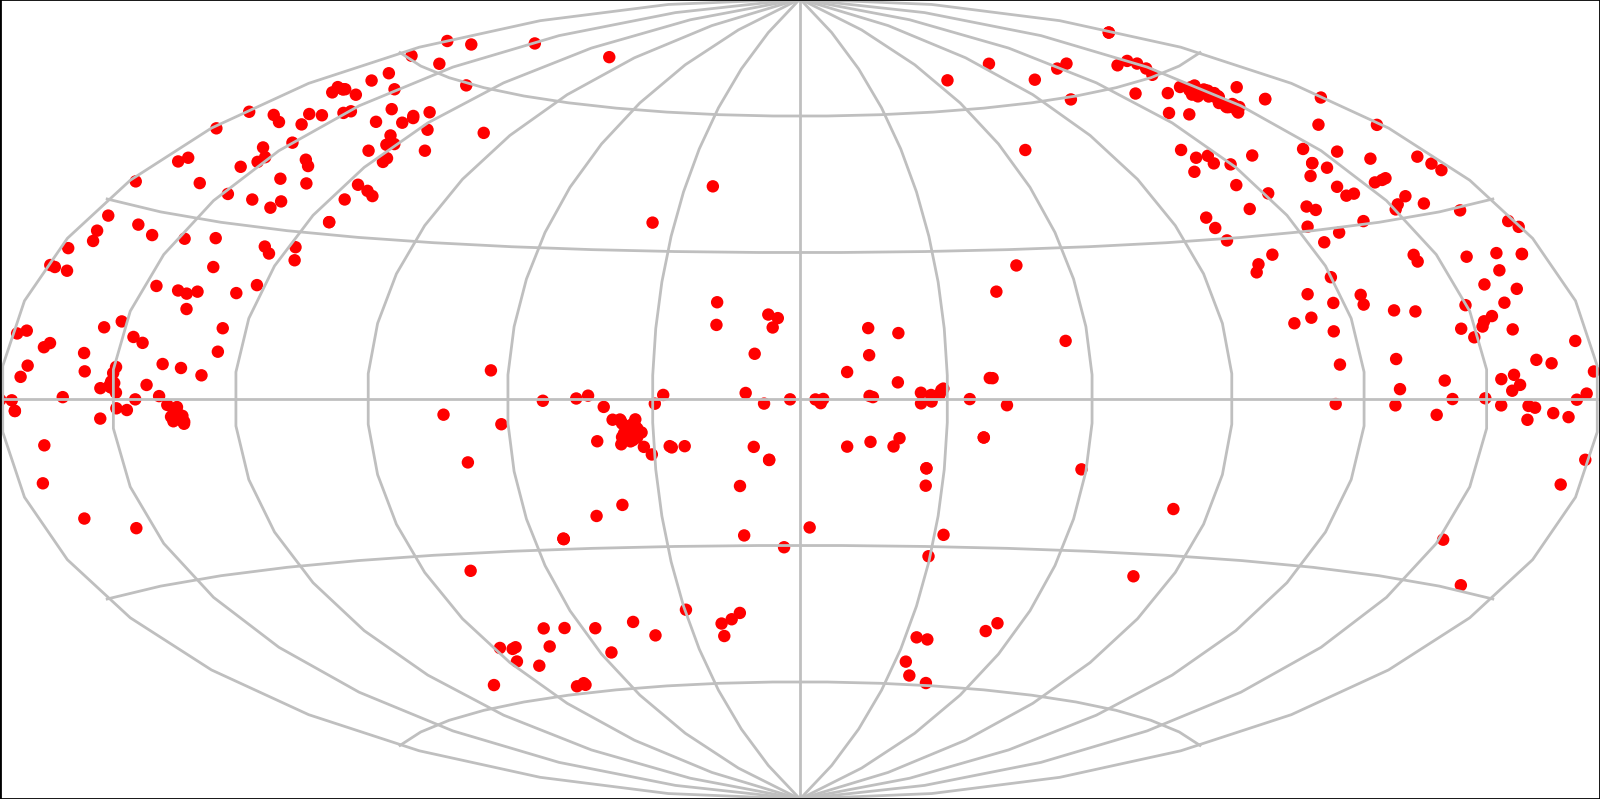
\includegraphics[width=\hsize]{fig/lenssky}
\caption{Sky distribution of 423 published lenses considered secure
  (from the Masterlens catalog at the University of Utah, maintained
  by Joel Brownstein and Leonidas Moustakas).  The map is in
  Hammer-Aitoff projection, with North up and $\rm RA=0$ in the
  middle. The empty swathes to the left and right of centre are the
  Milky Way. {\em Should we drop this figure?  It's not relevant to
    modelling, but as there seems to be no publicly available summary
    of all known lenses, it does help set context.}}
\label{fig:masterlens}
\end{figure}

Surveys now under way aim to increase the inventory of lenses another
ten or a hundred fold.  Among these is \sw (Marshall et al, in prep,
More et al, in prep).  \sw is a citizen science project\footnote{\tt
  http://www.spacewarps.org} in which volunteers are presented
sky-survey images and invited to identify lens candidates.  Simulated
lenses are mixed in with the data, both to help train volunteers on
what to look for, and to provide measures of the effectiveness of the
search.  The motivation for \sw is to enable volunteers, some of whom
had previously serendipitously identified lens candidates on earlier
citizen-science surveys, to make discoveries missed in automatic
searches by software robots.  Robots are very good with clean lensing
system in uncrowded fields with high signal-to-noise, but in general
test situations \citep{2009ApJ...694..924M} robots miss lenses (low
completeness) or contaminate the results with non-lenses (low purity).
\sw introduced its first tranche of survey data, in May 2013, from the
Canada-France-Hawaii Telescope Legacy Survey (CFHTLS), covering
$\simeq172$ square degrees (0.4\% of the sky) was divided into tiles
of $\simeq 80''\times80''$ ($440\times 440$ pixels).  Each such tile
was shown to ten volunteers.  Despite the rarity of detectable lenses
($<10^{-3}$ per tile), the \sw collective soon found lens candidates,
both rediscoveries already known from robots \citep{Gavazzi2012,
  More2012ApJ} and possible new lenses.

The encouraging early results prompted the question: could modeling of
the lenses also be done by volunteers?  There are several software
tools for lensing modelling available, and work has been done on
generic interfaces \citep{2013NewAR..57....1L,2014A&C.....5...28L}.
Some early designs for \sw included a prototype lens modelling tool
\citep{2010AAS...21543527N}.  Moreover, some {\em Spacewarps\/}
volunteers are quite experienced from earlier projects, having spent a
thousand hours or more with data, and are very interested in more
demanding projects.  The interests of citizen-science communities are
just beginning to be studied \citep[e.g.,][]{2013AEdRv..12a0106J}, but
it is clear that some volunteers welcome open-ended challenges, and
sometimes these have led to new scientific results: one example is the
discovery of an exceptional extra-solar planet
\citep{2013ApJ...768..127S}; another is the development of new
algorithms for protein folding \citep{Khatib22112011}.  All these are
grounds for optimism.  There is, however, a basic difficulty in strong
gravitational lensing.  Lensed images do not look much like their
source, and still less do they resemble the lensing-mass distribution.
To model a lens, one needs to either do a lot of random guessing, or
have a good intuition for what works.

In this paper, we propose a way around the difficulty, and report on a
modelling test on \sw using simulated lenses.  The three following
sections are devoted to the concept, the implementation, and tests
respectively.

In \secref{Fermat} we introduce a markup system for lensed images,
which we call a ``spaghetti diagram''.  A spaghetti diagram resembles
the visible image system, in a cartoon-like way, and at the same time
it encodes the basis of a mass model.  This supplies an intuitive link
between the image system and the mass distribution, which look
frustratingly different from each other.  Spaghetti diagrams are
essentially the saddle-point contours originally introduced to
gravitational lensing by \cite{1986ApJ...310..568B} as a way of
classifying lensed images.  They are sometimes shown as part of the
output of lens models \citep[for
  example][]{2001ApJ...557..594R,2003ApJ...590...39K,Lubini2012}.  In
the present work, however, spaghetti diagrams are the {\em input\/}
through which the modeller tells the program what to do.

In \secref{SpaghettiLens} we describe the \spl program, which
implements everything.  \spl is an extension of the GLASS framework
for modelling lenses \citep{2014arXiv1401.7990C}.  We will not go into
software details in this paper, concentrating instead on lens
modelling per se, but we remark that \spl is designed to be friendly
to the forum style of citizen-science projects, without sacrificing
any features of GLASS.  The program is invoked online, and the
modelling history is logged in a transparent way, enabling forum
discussions and incremental improvement by different people.
Moreover, any result can be revisited and post-processed if desired.

In \secref{mod_challenge} we describe a modelling challenge where a
diverse sample of 29 simulated lenses was modelled multiple times
using \spl.  The models are then examined in two ways.  One was
whether the spaghetti diagram was correct.  The other was the recovery
of the Einstein radius.  In addition, we show some visual comparisons
of actual and recovered lens shape and radial profile, and identify
some areas to improve, but do not compute statistics on these aspects.
Profile and shape recovery with GLASS has been studied in more detail
in \citep{2014arXiv1401.7990C}.

\secref{todo} concludes, with the general outlook and next steps.

\section{Fermat's principle and spaghetti diagrams} \label{sec:Fermat}

\subsection{Geometrical and gravitational time delays} 

Let us recall the formulation of gravitational lensing by
\cite{1986ApJ...310..568B} in terms of Fermat's principle.  Consider a
lens at some redshift $z_L$ and let $(x,y)$ be planar coordinates at
the lens, transverse to the line of sight.  Let $\Sigma(x,y)$ be the
mass per unit area, i.e., density projected along the line of sight.
This surface density is often given in a dimensionless form
\begin{equation} \label{eq:kappa}
\kappa(x,y) \propto \Sigma(x,y)
\end{equation}
called the convergence.  And let there be light, in the form of a more
distant source, at redshift $z_S$, behind point $(x_s,y_s)$ on the
lens.

We now imagine a virtual photon flying from the source to some $(x,y)$
on the lens, then changing direction and coming to the observer.  Such
a direction change would increase the light travel time compared to
coming through $(x_s,y_s)$.  The increased light travel time from the
geometry of deflection would be
\begin{equation} \label{eq:tgeom}
\tgeom(x,y) \propto (x-x_s)^2 + (y-s_y)^2 \,.
\end{equation}
assuming the delay is small compared to the total light travel time.

An additional delay of the photon comes from travelling through the
curved spacetime at the lens, and can be related to the mass
distribution of the lens by an implicit relation, as follows.  The
value of $\tgrav$ through $(x,y)$ equals its average value on the
circumference of a small circle centred at $(x,y)$, plus a constant
times the mass within that circle.  The proportionality constant is
$2G/c^3$ times the cosmological expansion factor $(1+z_L)$. Thus
\begin{equation} \label{eq:tgrav}
\tgrav(x,y) = \left\langle \tgrav(x_\subcirc,y_\subcirc) \right\rangle
              + (1+z_L) \frac{2G}{c^3} M(x_\subbullet,y_\subbullet) \,.
\end{equation}
We have used $(x_\subcirc,y_\subcirc)$ to denote the circumference of
a circle, and $(x_\subbullet,y_\subbullet)$ to indicate the integrated
mass within the circle.

The light travel time of a virtual photon is therefore longer by
\begin{equation}  \label{eq:tarriv}
t(x,y) = t_{\rm geom} + t_{\rm grav} \,.
\end{equation}
than it would have been with no lens present.  Real photons take paths
that make $t(x,y)$ extremal, that is, having a minimum, maximum or
saddle point (Fermat's principle).

The proportionality factors in \eqref{eq:kappa} and \eqref{eq:tgeom}
depend on the redshifts and cosmological parameters, and are given in
the Appendix~\ref{more-theory}.

\begin{figure}
\centering
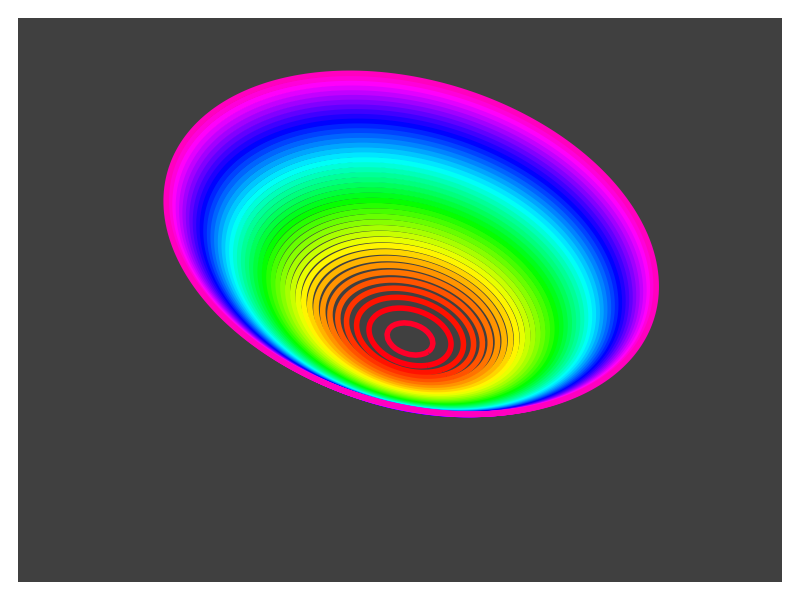
\includegraphics[width=\columnwidth]{fig/arriv_0}
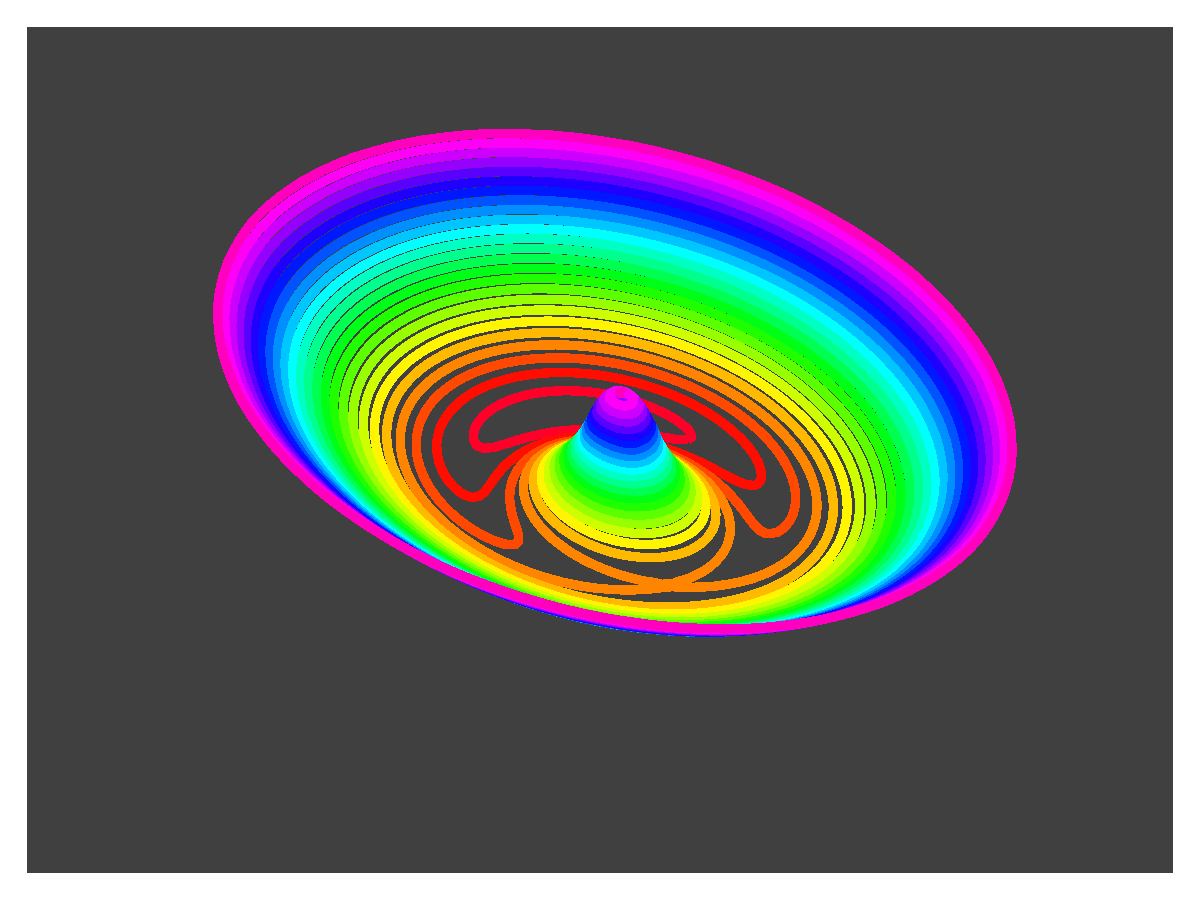
\includegraphics[width=\columnwidth]{fig/arriv_1}
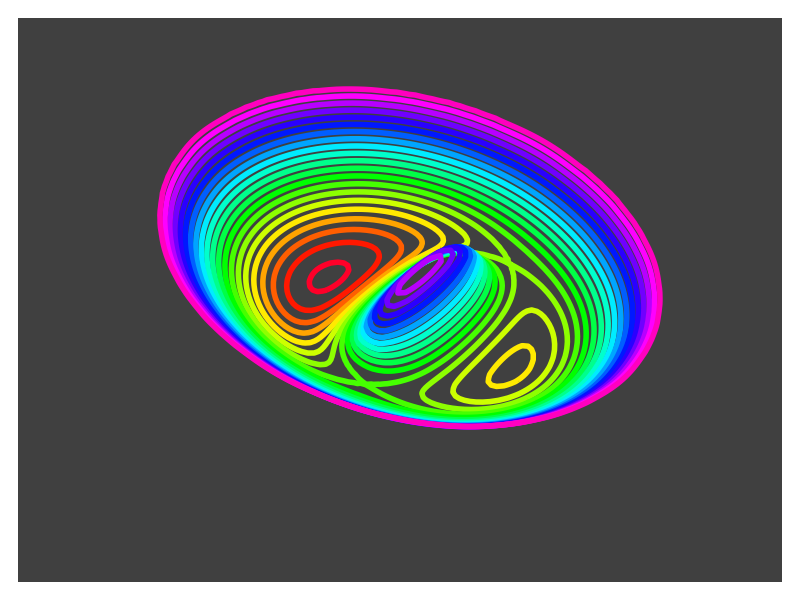
\includegraphics[width=\columnwidth]{fig/arriv_2}
\caption{Perspective views and contour maps of example arrival time
  surfaces.  Contours are coloured in rainbow order (red: least delay,
  violet: highest delay).  {\em Upper panel:\/} No lens, hence showing
  the parabolic shape of the geometrical time delay.  The image would
  be at the bottom, coinciding with the source. {\em Middle panel:\/}
  A circular lensing mass (offset from the source) has been added,
  which has pushed the minimum to one side and introduced a maximum
  and saddle point, each corresponding to an image.  The saddle-point
  is characterized by a self-crossing ``spaghetti'' contour. {\em
    Lower panel:\/} An elongated lensing mass has been added.  There
  are now two minima, two saddle points, and a maximum, each
  corresponding to an image.  Note the two self-crossing spaghetti
  contours associated with the saddle points.}
\label{fig:arriv}
\end{figure}


\subsection{Arrival-time contours} \label{sec:arriv}

The full function $t(x,y)$, also known as the arrival-time surface,
applies to virtual photons.  In other words, it is an abstract
construct and not itself observable.  But observable image positions
can be derived from the arrival-time surface, so visualising the
surface is useful.  \figref{arriv} does so.  In this figure, a
maximum, if present, is easy to see.  To locate mimima and
saddle-points, however, one needs to examine the contours of equal
arrival time.  A saddle point is characterised by a contour crossing
itself, forming an~X.  Mimima, on the other hand, have contours
looping around them, as do maxima.

The saddle-point contours which form an X are especially interesting,
because they set the overall topography of the arrival-time surface.
The obviously give the locations of the saddle points, and roughly
localise the minima and maxima as well.  If more precise locations of
the minima and maxima are added, the whole arrival-time surface is
already approximately known.  Since the arrival-time surface has an
exact relation to the lens-mass distribution and the source position,
in effect the mass distribution is also automatically specified.  In
other words, a simple sketch of saddle-point contours along with
locations of minima and maxima ---which we call a spaghetti diagram---
is implicitly already an approximation to a lens-mass distribution.

The preceding assumes a point source.  To get an idea of what an
extended source would do, let us imagine moving the original source
slightly.  The contours of constant arrival time will naturally move
slightly, and so will the images.  The movement of the contours will
be most noticeable where the contours are far apart, that is where the
arrival-time surface is nearly flat.  As is evident from
\figref{arriv}, this is the region where the minimum and saddle points
lie, or near the images.  In this region, points on the source that
are close together produce images that are comparatively far apart.
In other words, the image is highly magnified.  In summary, lower
curvature in the arrival-time surface for a point source implies
larger magnification of an extended source.  Conversely, where the
arrival-time surface is strongly curved, the image will be
demagnified.  We see from \figref{arriv} that the arrival-time surface
tends to be highly curved near the maximum.  Hence maximum tend to be
demagnified.  In practice, maxima of the arrival time are nearly
always too faint to see. The minima and saddle points dominate.

\section{A lens-modelling program} \label{sec:SpaghettiLens}

Modelling with \spl involves three stages, markup of the image,
followed by intensive numerics in the background, followed by review
of diagnostics and possible discussion.  We now describe each of
these, but do not go into implementation details.

\subsection{Image markup}

One begins by going to the \spl page and entering the number of a \sw
image tile.  \spl presents the image, along with zoom and pan options
and a markup tool to construct a spaghetti diagram.  The human
modeller now has to make an educated guess for the topography of the
arrival-time surface, and input the locations time-ordering of the
maxima, minima, and saddle-points.  The markup tool \citep[which is
  inspired by Figure~6 of][and is like that figure made interactive
  and overlaid on data]{1986ApJ...310..568B} lets the modeller enter
the information by sketching saddle-point contours.  Examples can be
seen in the upper-left panels of Figures \ref{fig:6941} to
\ref{fig:7022}.  The loops in the markup tool were the origin of the
``spaghetti'' metaphor.

The exact placement of the loops in a spaghetti diagram has no
significance, only the connections, and the heirarchy of which loop is
inside which matters.  The loops are there simply to help modeller's
intuition.  The user does not need to think explicitly the image
parities (though the markup tool provides this information using
colour codes) or about time-ordering, or worry about the odd-image
theorem.  The markup tool allows only valid lensing configurations to
be entered.

As implemented so far, \spl assumes that the lens is dominated by a
single galaxy.  Only one maximum is permitted, and it is taken as the
centre of the main lensing galaxy.  The user can, however, mark
additional minor galaxies.  The latter are modelled as point
masses.

\subsection{Numerics}

Having sketched a spaghetti diagram, the user orders a model, and \spl
sends the input to GLASS, which runs server-side as it is
compute-intensive.  The task of GLASS is to find a mass distribution
$\kappa(x,y)$ that exactly reproduces the given locations of the
maximum, minima and saddle points. Now, this criterion by itself is
extremely under-determined --- there are infinitely many mass
distributions that will reproduce a given set of maxima, minima and
saddle points, but typically they (a)~produce lots of extra images,
and (b)~look very unlike galaxies.  Additional assumptions (a prior)
are necessary.  GLASS uses the following prior
\citep[cf.]{1997MNRAS.292..148S,2008ApJ...679...17C}.
\begin{enumerate}
\item The mass distribution is built out of non-negative tiles of
  mass.  (Sometimes these tiles are called mass pixels, but we should
  emphasize that they are unrelated to image pixels, and are much
  larger.)
\item There is a notional lens center, say $(x_0,y_0)$ which is
  identified with the maximum of the arrival time.  The source can
  have an arbitrary offset with respect to the lens center.
\item The mass distribution must be centrally concentrated, in two
  respects.  First, the circularly averaged density must fall away
  like $$ \left[(x-x_0)^2+(y-y_0)^2\right]^{-1/2}$$ or more steeply.
  Second, the direction of increasing density at any $(x,y)$ can point
  at most $45^\circ$ away from $(x_0,y_0)$.
\item The lens must be symmetrical with respect to $180^\circ$ rotations
  about $(x_0,y_0)$.  This symmetry assumption can be relaxed if the
  user wishes.
\end{enumerate}
There are still infinitely many models that satisfy both data and
prior constraints, but now they are more credible as galaxy lenses.
It is then possible to generate an ensemble of models.  The sampling
technique used by GLASS is described in \citep{Lubini2012}.
Typically, ensembles of 200 models are used.  That is to say, what we
call a \spl model is really the mean of an ensemble of 200 models, and
its estimated uncertainty is the range covered by the whole ensemble.

\subsection{Diagnostics}

After the model ensemble has been generated, \spl post-processes it to
present results and diagnostics to the user for inspection. This takes
the form of three figures.
\begin{enumerate}
\item A synthetic image of the lensed features.
\item A contour map of the arrival-time surface $t(x,y)$.
\item A gray scale plus contour map of the mass distribution.
\end{enumerate}
The synthetic image generated by \spl assumes a simple conical source
profile.  The user can change the contrast level on the image, which
(though it is not saved) amounts to adjusting the width of the cone.
These synthetic images are still very crude and not very useful for
assessing models.  The best indicator, in practice, of whether the
modelling was successful is contour map of $t(x,y)$, with saddle-point
contours highlighted.  It is, in effect, the computer's refinement of
the spaghetti diagram input by the user.  If the arrival-time surface
looks qualitatively similar to the spaghetti diagram, that generally
indicates a successful model.  The mass distribution also provides
indications; successful models generally lead to smooth-looking mass
distribution, whereas an irregular or checkboard pattern in the mass
map signals a bad model.

After examining this feedback, the user can choose to post the model
on the \spl archive.  They can also modify their input and try again,
or discard the attempt altogether.  After archiving, there can be
discussion among modellers, through the \sw forum or by any other
means, and revision of the model.  Any archived model can be revised
by any user: they can modify the spaghetti configuration slightly or
drastically, or change options like the size of the mass tiles.
Particularly interesting lens candidates lead to trees of models in
this way.  Discussion among modellers tends to prune a model tree,
focusing attention on the most interesting models.\footnote{See
  ``Collaborative gravitational lens modelling\dots'' in {\tt
    http://letters.zooniverse.org} for an example.}

\section{A lens modelling challenge} \label{sec:mod_challenge}



Once an early version of \spl

Through the SW discusison forum (TALK), we asked active members of the Space Warps Citizen community for interest in modelling lens systems. XX interested users volunteered to perform modelling and were introduce

Interested volunteers from the \sw forum were initially introduced to
\spl through a video tutorial and by videocon.  After this
introductory stage, a modeling challenge was presented.  This
consisted of 29 simulated lenses (sims) covering a range of lensing
configurations.

The \sw sims were generated by AM, in consultation with PM and AV.
To estimate the performance of the volunteers and the quality of the generated models, two analysis  were done.
The first analysis tested the correct identification and ordering of lensed images.
The second one compared the mass distribution of the lens $\kappa(x, y)$ of the generated models to the mass distribution of the simulations.

A challenge set of 29 was selected, representing the different image
morphologies among the spacewarps sims.  Modellers then contributed
129 models for these sims (at least for each sim).  Models were
collecting in the same forum used to model real candidate lenses, and
under the same conditions --- modellers were free to consult and
refine each other's models, but had no information on how the sims
were generated.

\subsection{The simulated lenses} \label{sec:sims}

The sims were produced using {\tt gravlens}
\citep{2001astro.ph..2341K,2001astro.ph..2340K} using the CFHTLS survey data
and catalogues \cite{Coupon2009}. They were of three
kinds, as follows.

\begin{enumerate}
  \item Imitating lensed quasars: having a singular elliptical
    isothermal lens (SIE) plus constant external shear, and a circular
    Gaussian source.
  \item Emulating lensed galaxies: similar to the above, but with an
    elliptical de Vaucouleurs source.
  \item Resembling cluster lenses: having a source as above, but a
    more complicated lens, with one dominant elliptical SIE and
    one or more perturbing elliptical SIEs, plus a circular NFW
    \citep{1996ApJ...462..563N,1997ApJ...490..493N} to represent
    the underlying dark matter distribution.
\end{enumerate}

Formulas for the lenses appear in \cite{2001astro.ph..2341K}. The SIE
lenses follow equations (33--35) of that work, with core radius set to
zero.  The NFW lens is in equations (48) and (50), while shear is the
$\gamma$ term in equation (76).

The information in this section was not revealed to the person
choosing the challenge set (RK) or to the modellers (EB, CC, CM, PS,
JO and JW) until the modeling stage was done.

\subsection{Some example models} \label{sec:example_models}

The modellers proposed a total of 129 models for the 29 sims in the
challenge. Typically XX models were produced per simulation, with XX
systems having only XX models (corresponding tot he most simplest
simulations) to XX having XX models (a complex and contrversial lens
system). In the following we discuss eight example lenses in detail
with individual notes per system and corresponding plots are shown in
figures 4-11 (or whatever compact version you end up making). These
eight examples were chosen on the basis of …??

The modelers proposed a total of 129 models for the 29 sims in the
challenge.  Figures \ref{fig:6941} to \ref{fig:6919} show eight of
models in some detail.

\FloatBarrier

\begin{figure}
  \centering
  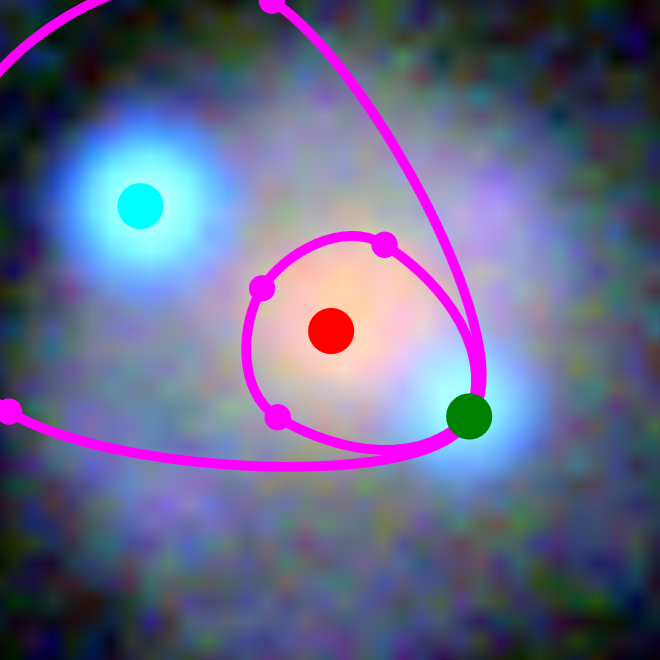
\includegraphics[width=\myplotswidth]{fig/006941_input}
  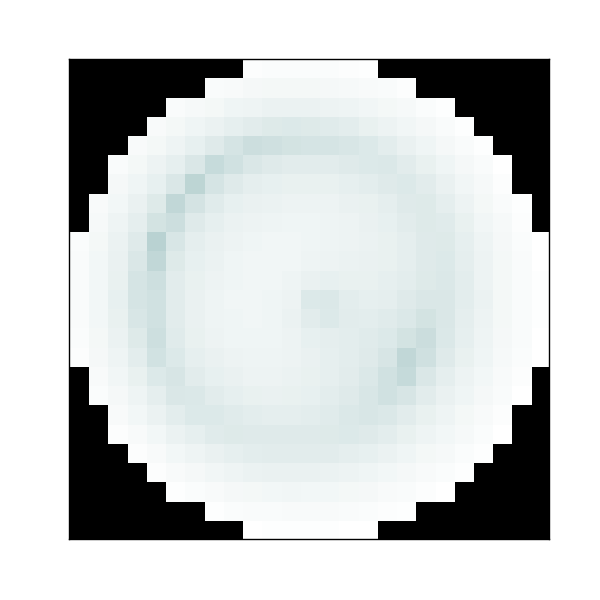
\includegraphics[width=\myplotswidth]{fig/006941_arr_time} \\
  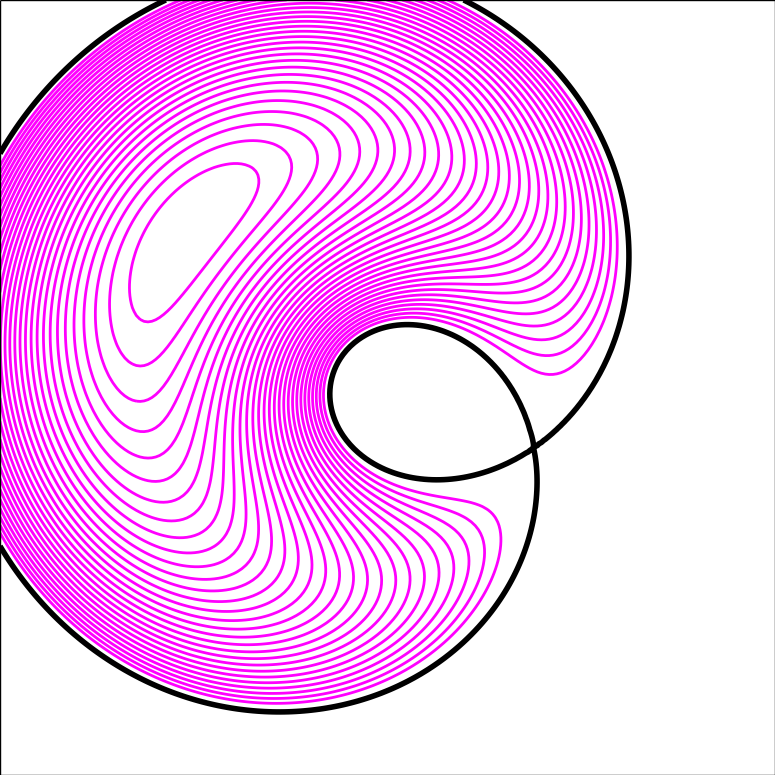
\includegraphics[width=\myplotswidth]{fig/ASW000102p_006941_arriv} 
  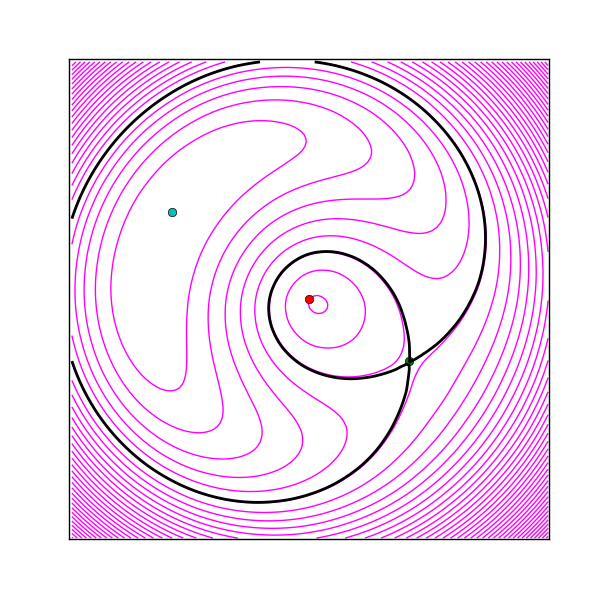
\includegraphics[width=\myplotswidth]{fig/006941_spaghetti} \\
  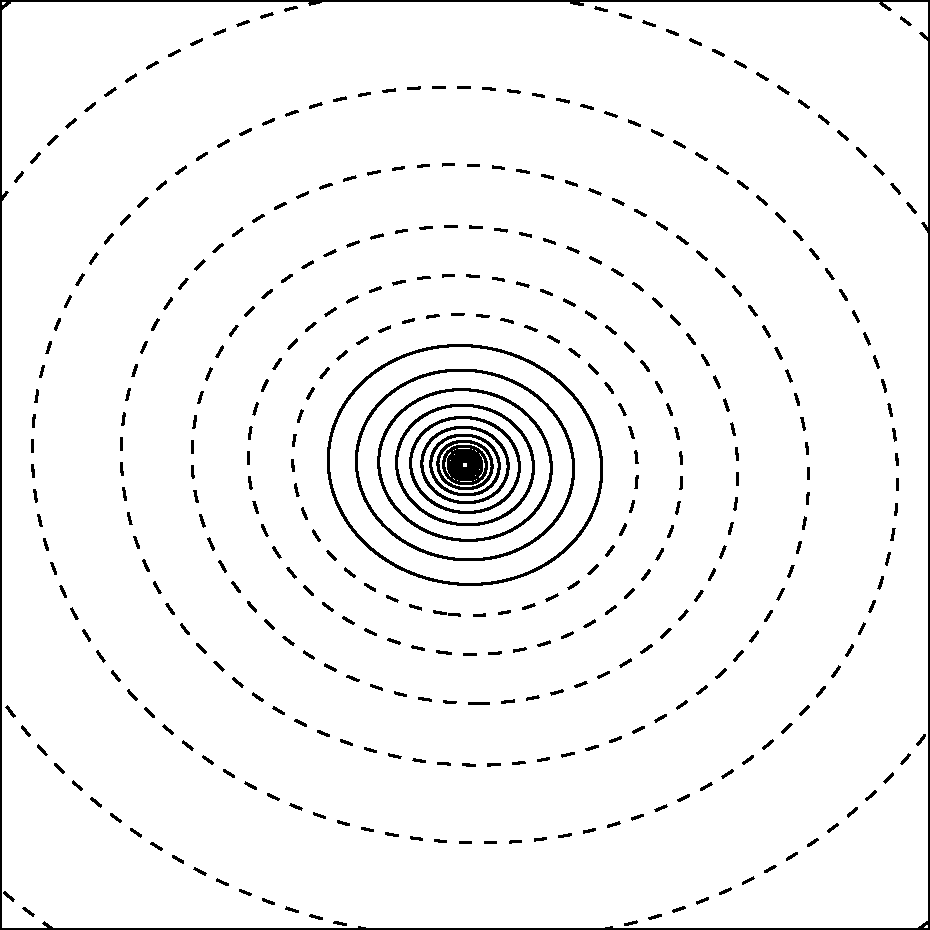
\includegraphics[width=\myplotswidth]{fig/ASW000102p_006941_kappa}
  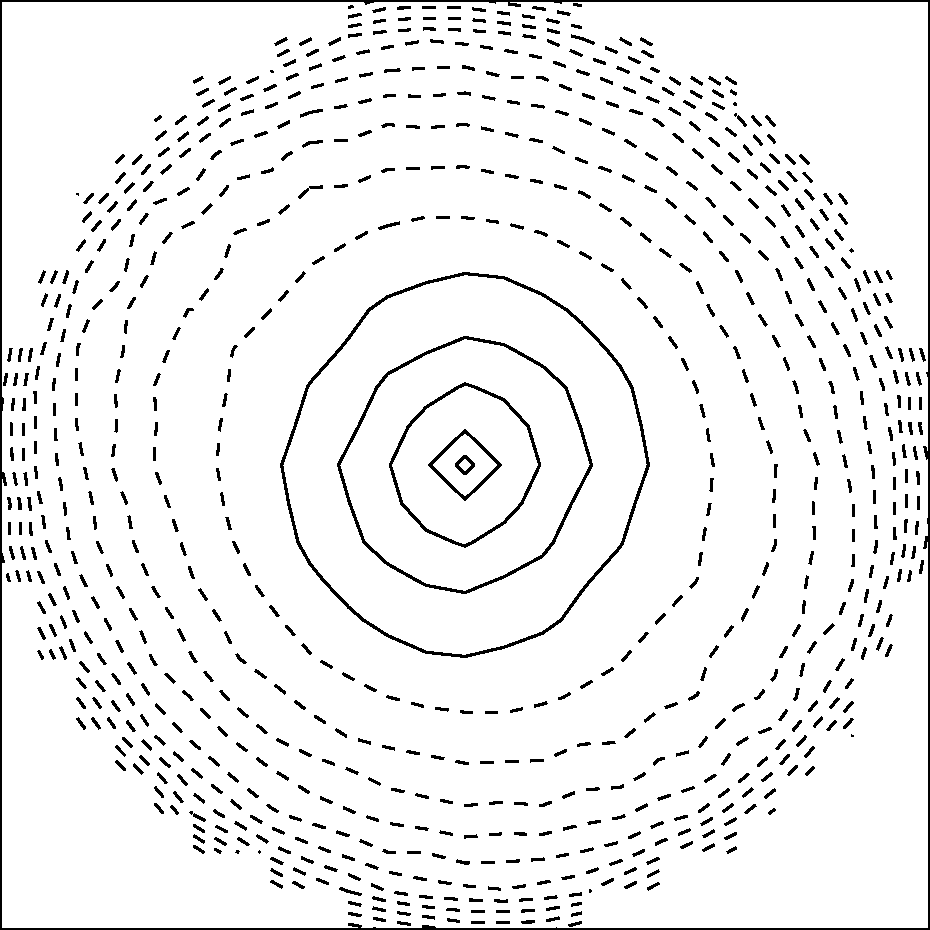
\includegraphics[width=\myplotswidth]{fig/006941_mass}
  \caption[result 6941 (ASW000102p)]{A simulated lens that mimics a
    lensed quasar, and model results.  The left panels derive from the
    simulation, and the right panels are \spl output.  Details of
    individual panels are in \ref{sec:example_models}.}

  \label{fig:6941}
\end{figure}

\begin{figure}
  \centering

  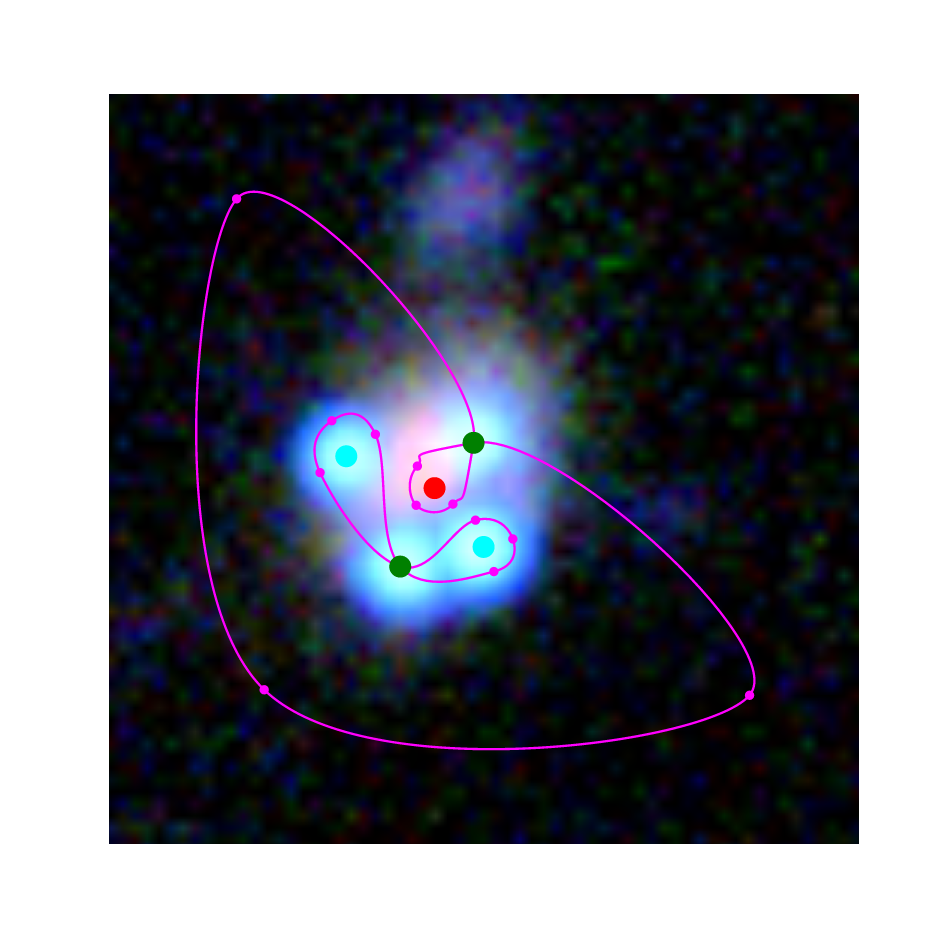
\includegraphics[width=\myplotswidth]{fig/006915_input}
  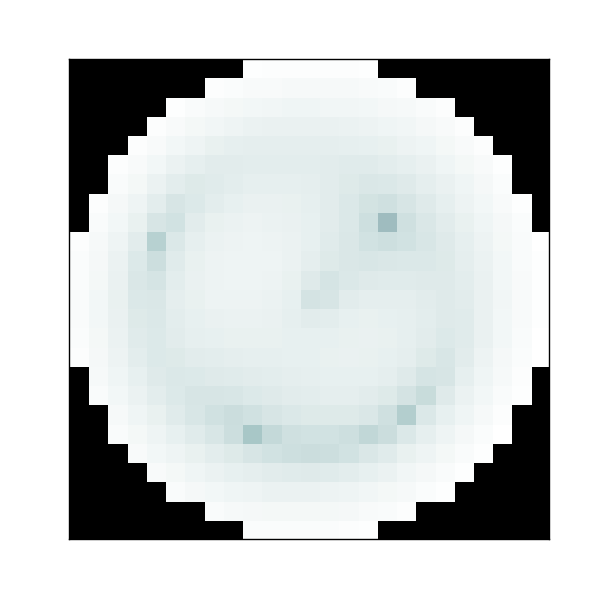
\includegraphics[width=\myplotswidth]{fig/006915_arr_time} \\
  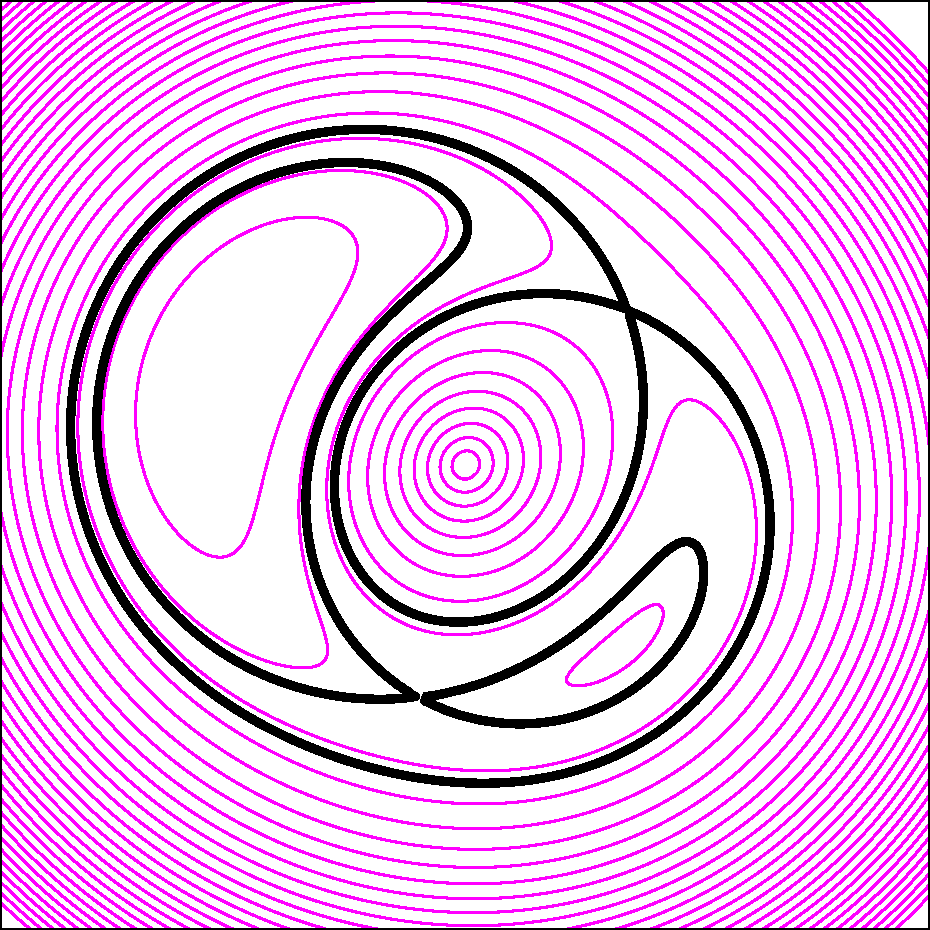
\includegraphics[width=\myplotswidth]{fig/ASW0001hpf_006915_arriv}
  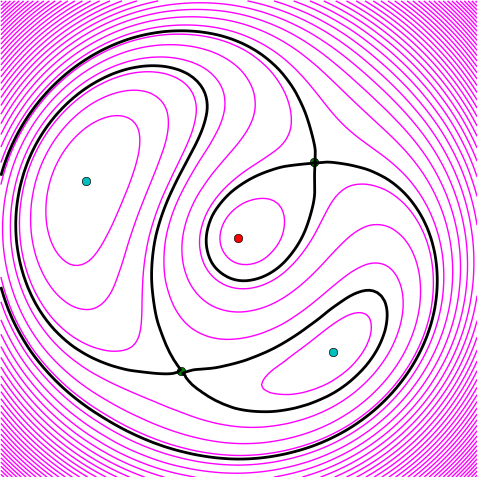
\includegraphics[width=\myplotswidth]{fig/006915_spaghetti} \\
  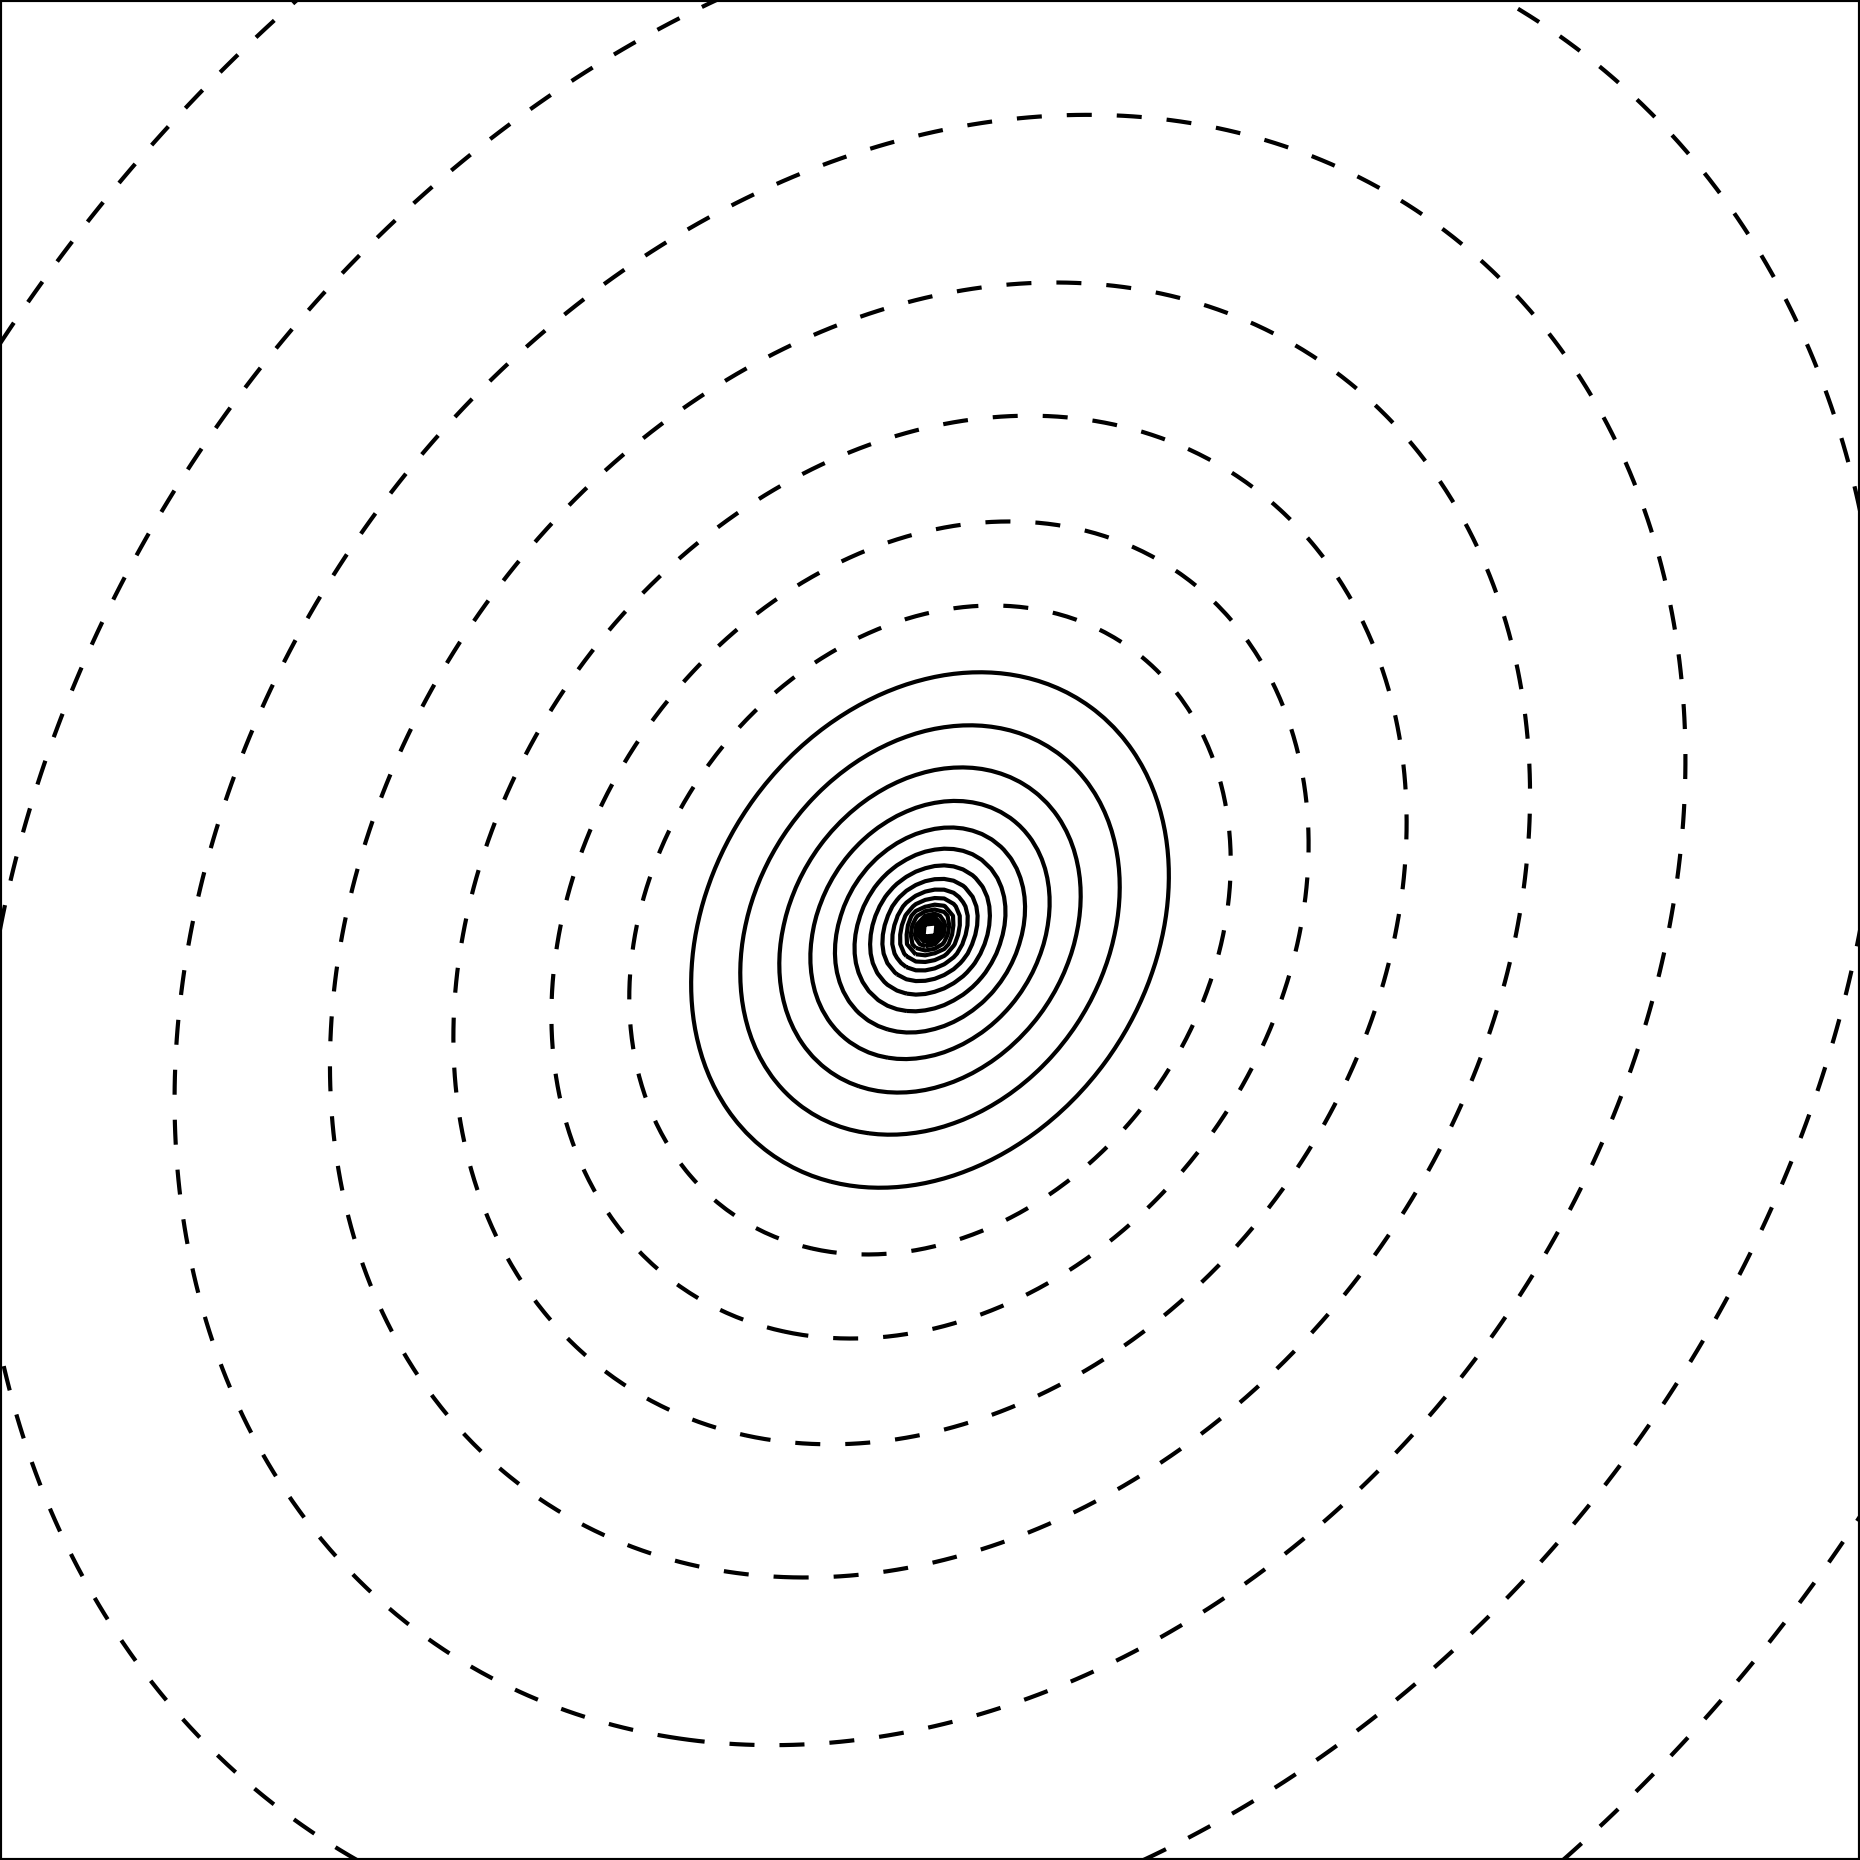
\includegraphics[width=\myplotswidth]{fig/ASW0001hpf_006915_kappa}
  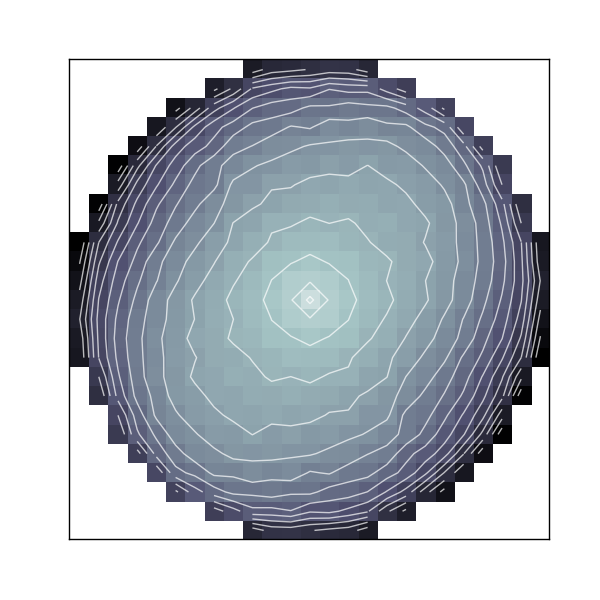
\includegraphics[width=\myplotswidth]{fig/006915_mass}

  \caption[result 6915 (ASW0001hpf)]{A four-image configuration
    typical of lensed quasars. (See Section \ref{sec:example_models}
    for details.)}
  \label{fig:6915}
\end{figure}


\begin{figure}
  \centering
  
  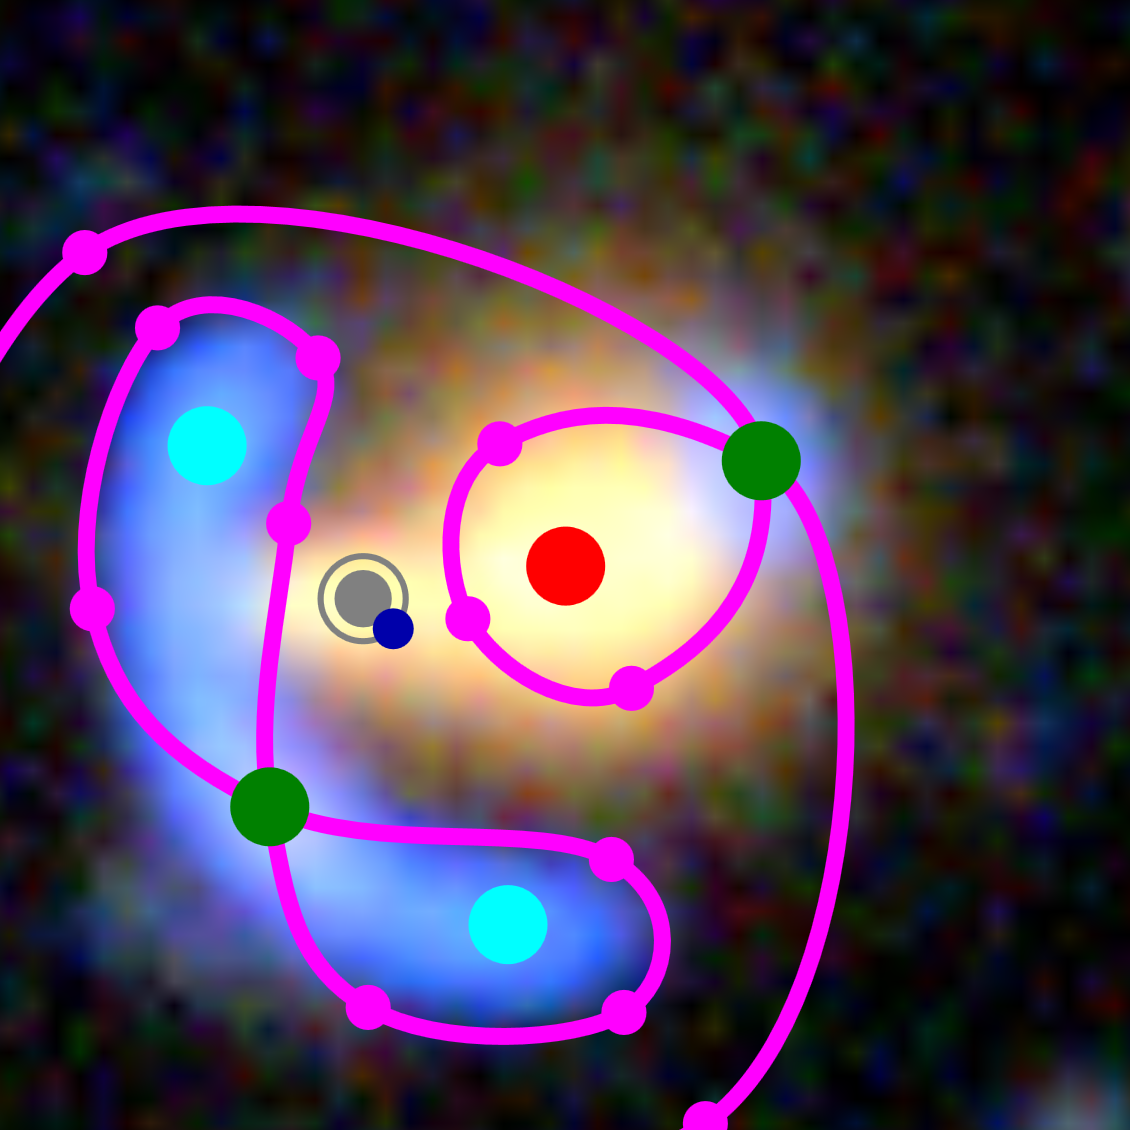
\includegraphics[width=\myplotswidth]{fig/006990_input}
  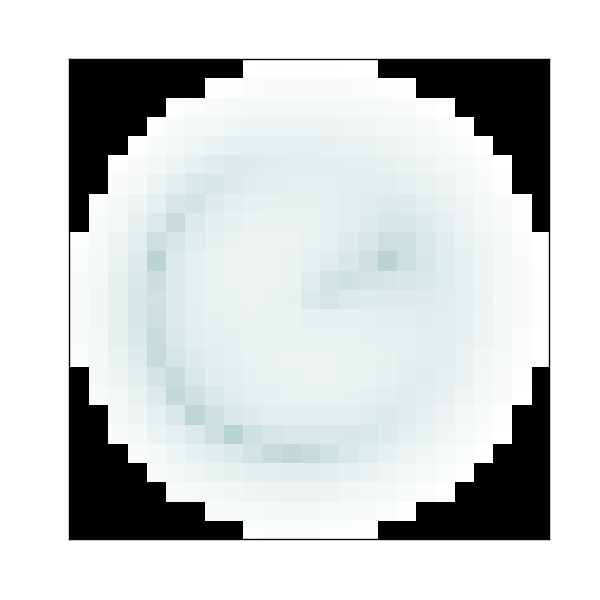
\includegraphics[width=\myplotswidth]{fig/006990_arr_time} \\
  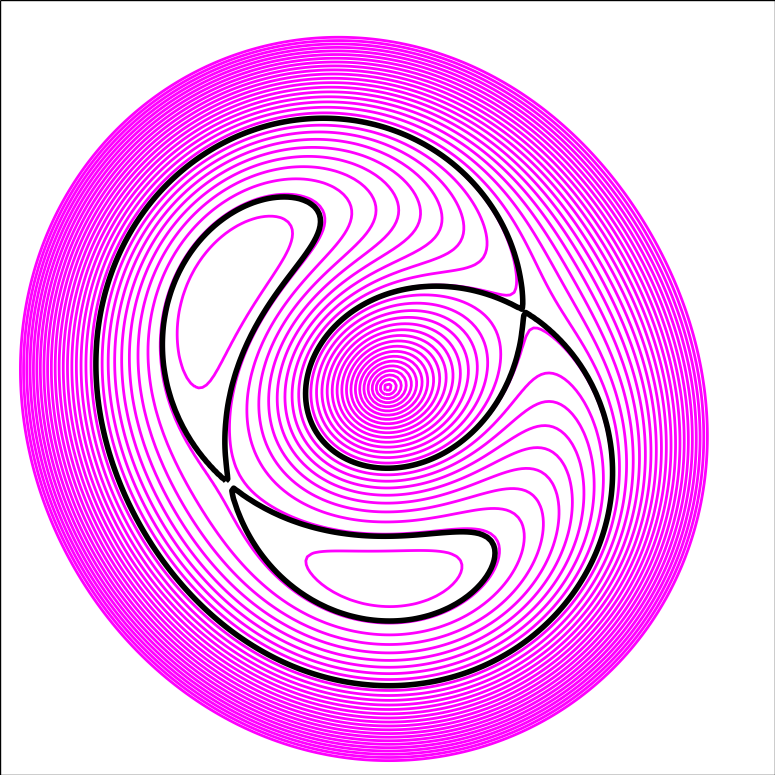
\includegraphics[width=\myplotswidth]{fig/ASW0004oux_006990_arriv}
  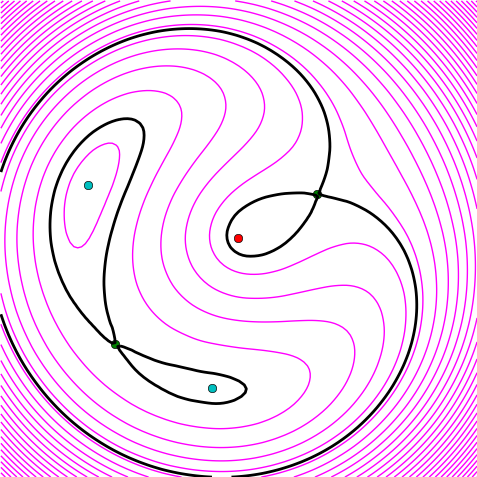
\includegraphics[width=\myplotswidth]{fig/006990_spaghetti} \\
  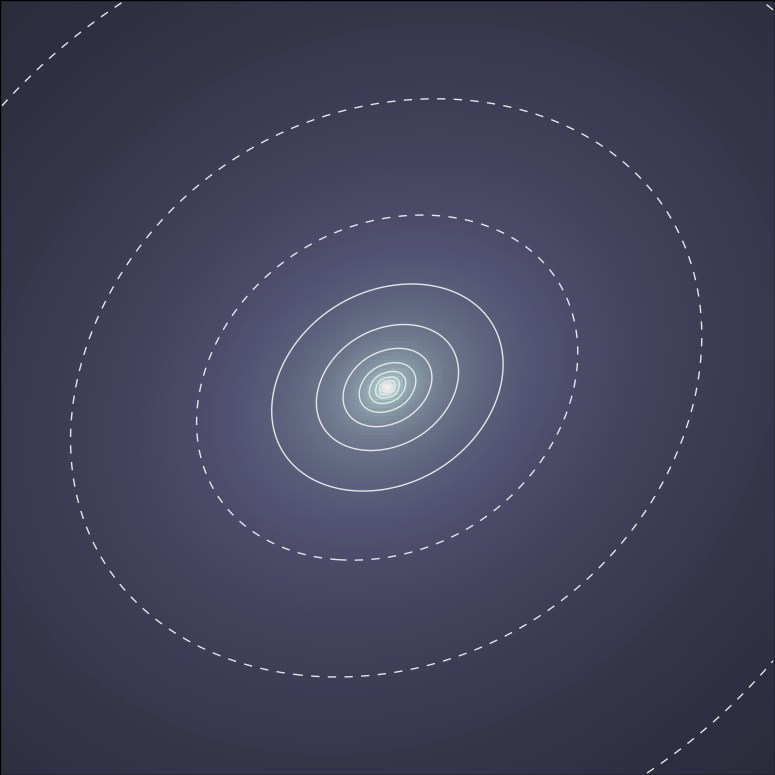
\includegraphics[width=\myplotswidth]{fig/ASW0004oux_006990_kappa}
  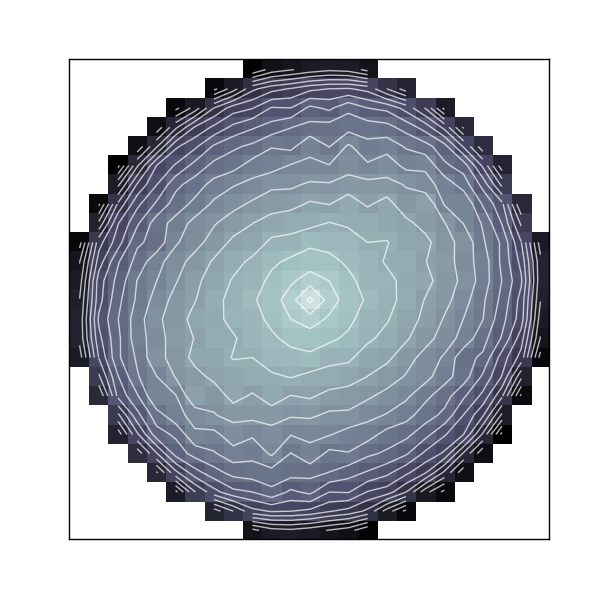
\includegraphics[width=\myplotswidth]{fig/006990_mass}

  \caption[result 6990 (ASW0004oux)]{Results from a system with an arc
    plus a counter-image, typical of lensed galaxies. (See Section
    \ref{sec:example_models} for details.)}
  \label{fig:6990}
\end{figure}



\begin{figure}
  \centering

  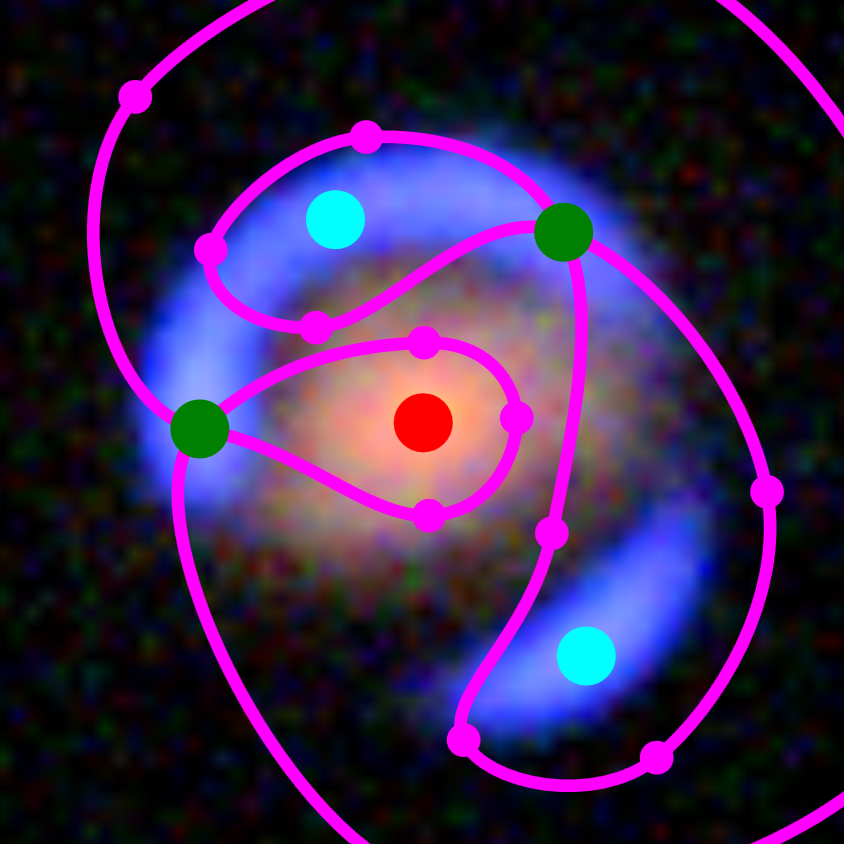
\includegraphics[width=\myplotswidth]{fig/006919_input}
  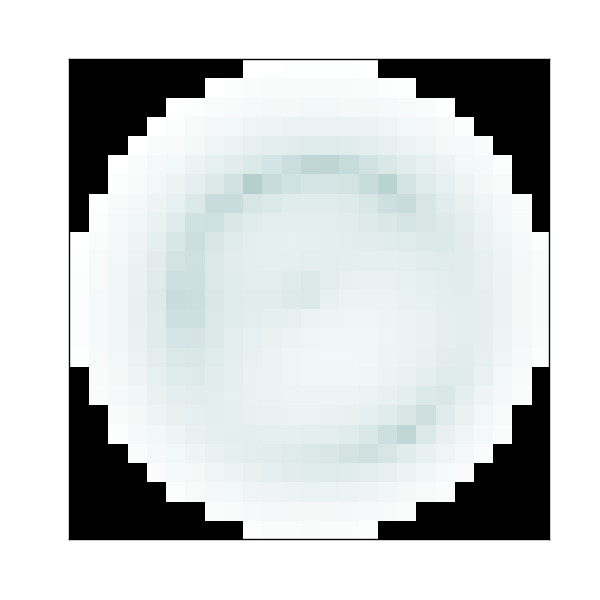
\includegraphics[width=\myplotswidth]{fig/006919_arr_time} \\
  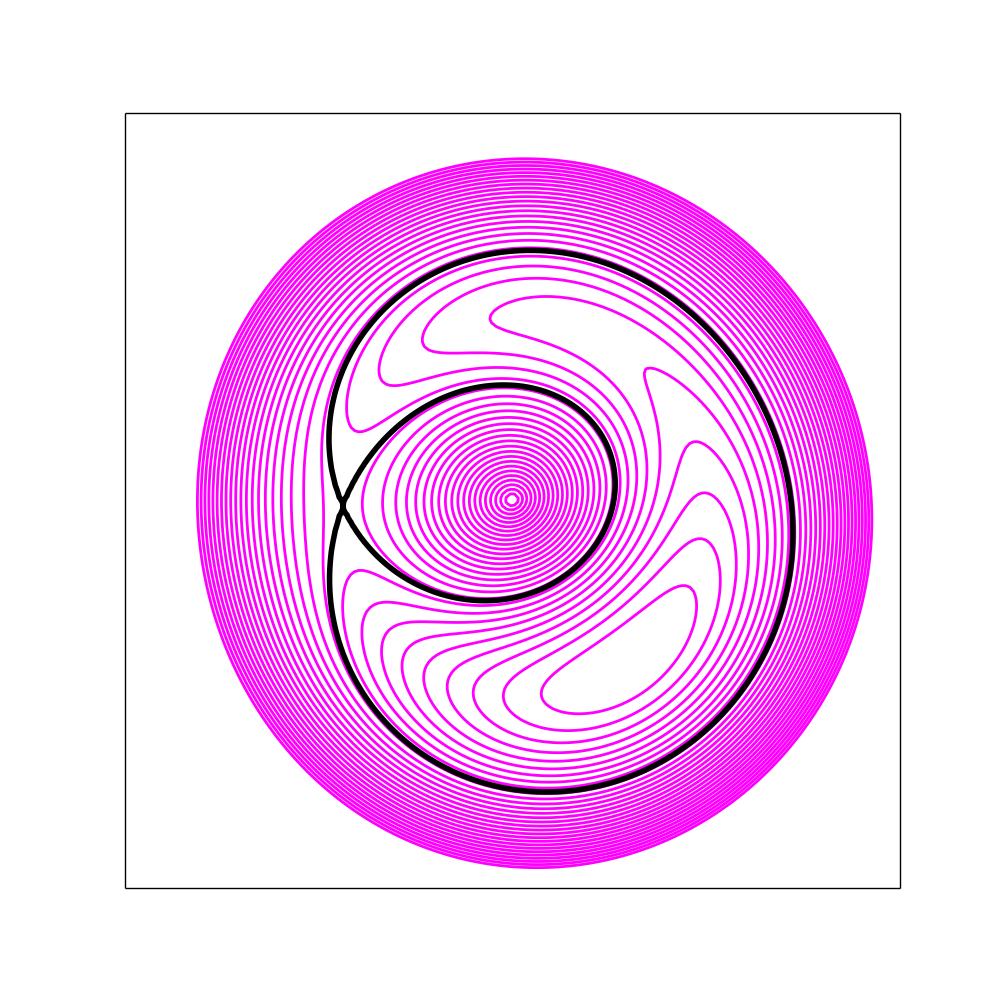
\includegraphics[width=\myplotswidth]{fig/ASW0002z6f_006919_arriv}
  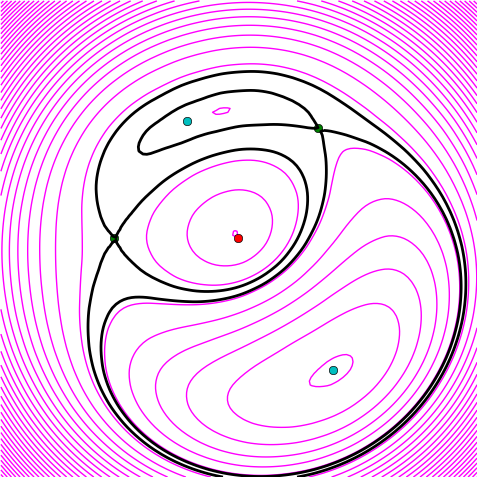
\includegraphics[width=\myplotswidth]{fig/006919_spaghetti} \\
  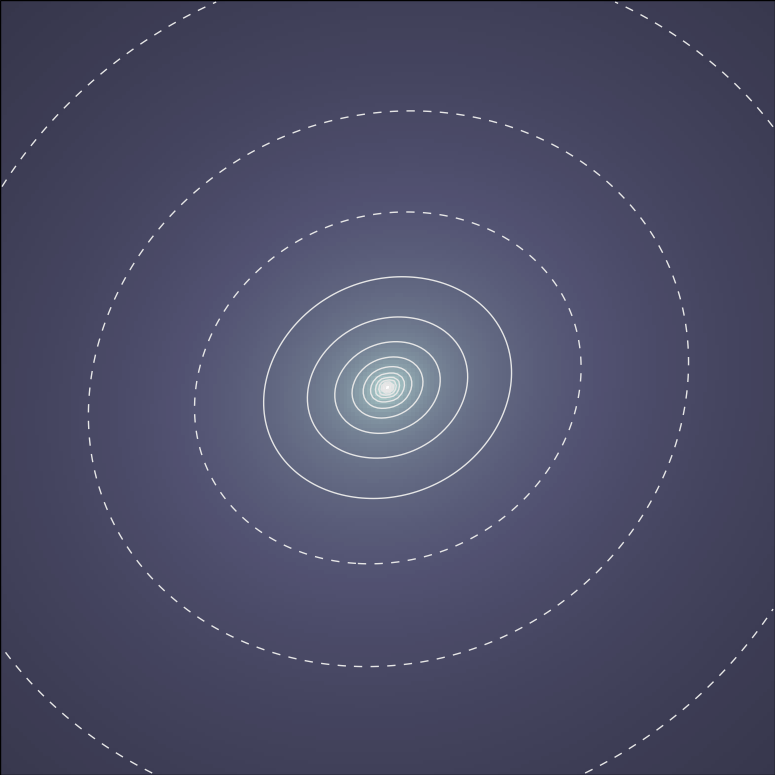
\includegraphics[width=\myplotswidth]{fig/ASW0002z6f_006919_kappa}
  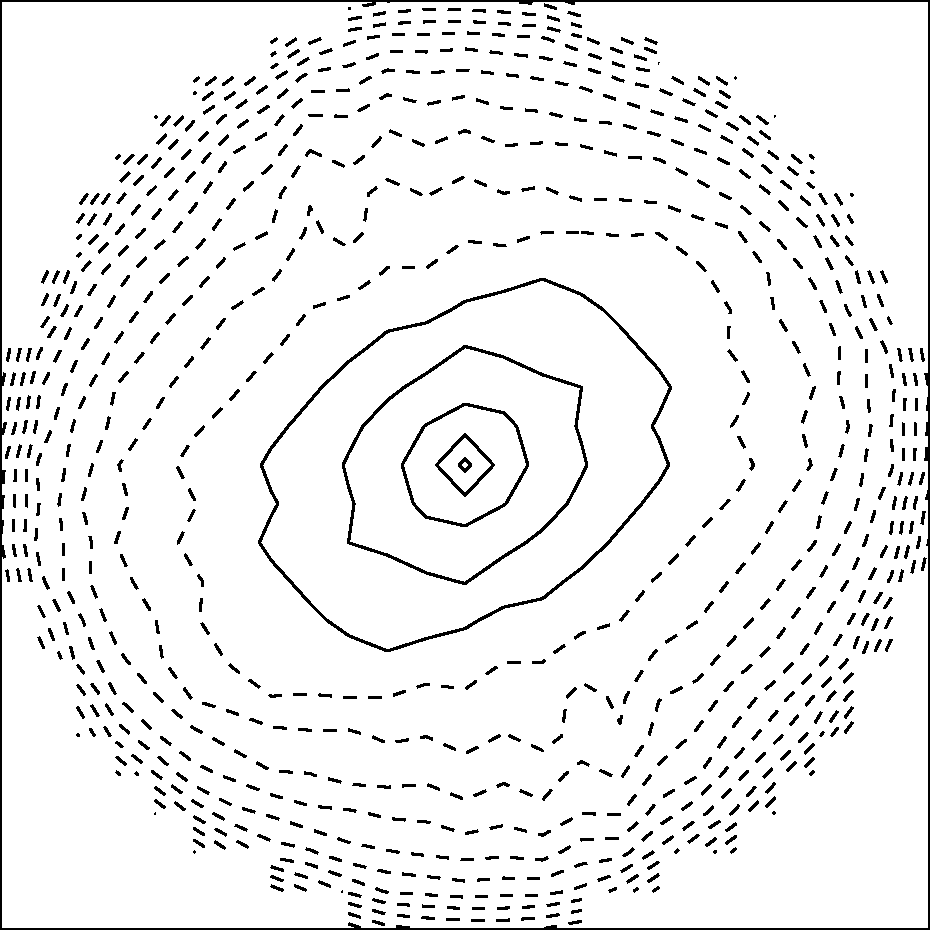
\includegraphics[width=\myplotswidth]{fig/006919_mass}

  \caption[result 6919 (ASW0002z6f)]{Another configuration of arc plus
    counter-image; here the arc is closer to the lensing galaxy than
    the counter-image. (See Section \ref{sec:example_models} for
    details.)}
  \label{fig:6919}
\end{figure}



\begin{figure}
  \centering
  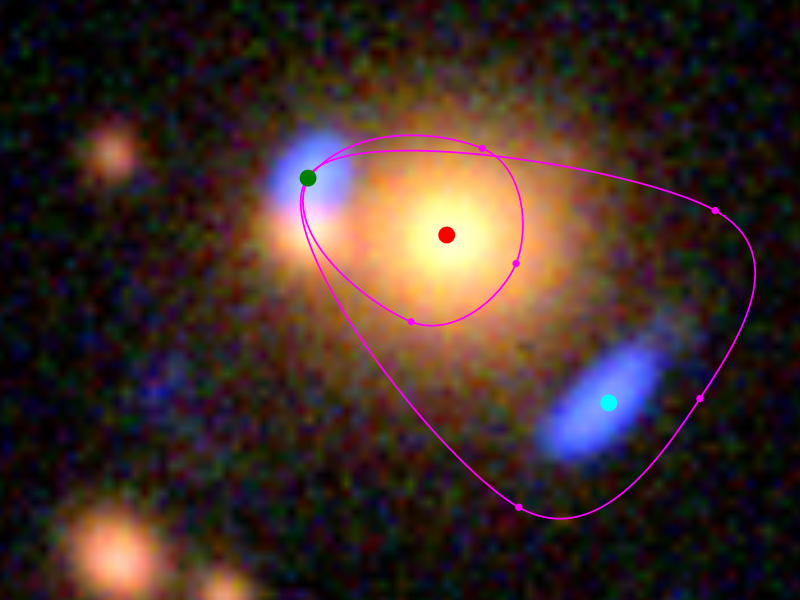
\includegraphics[width=\myplotswidth]{fig/006975_input}
  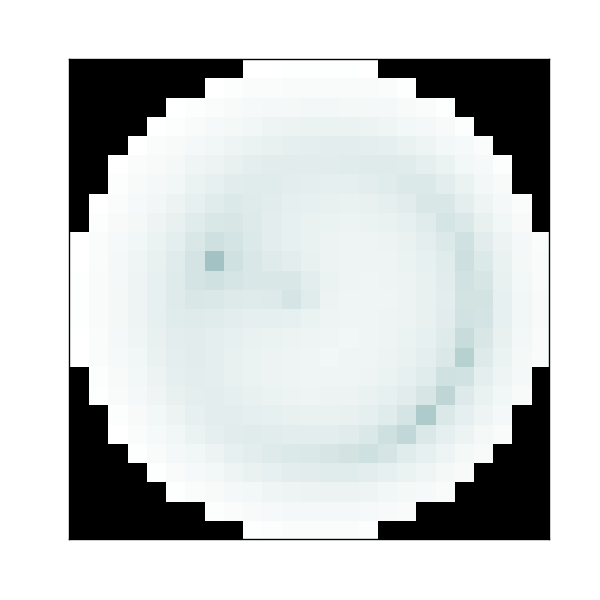
\includegraphics[width=\myplotswidth]{fig/006975_arr_time} \\
  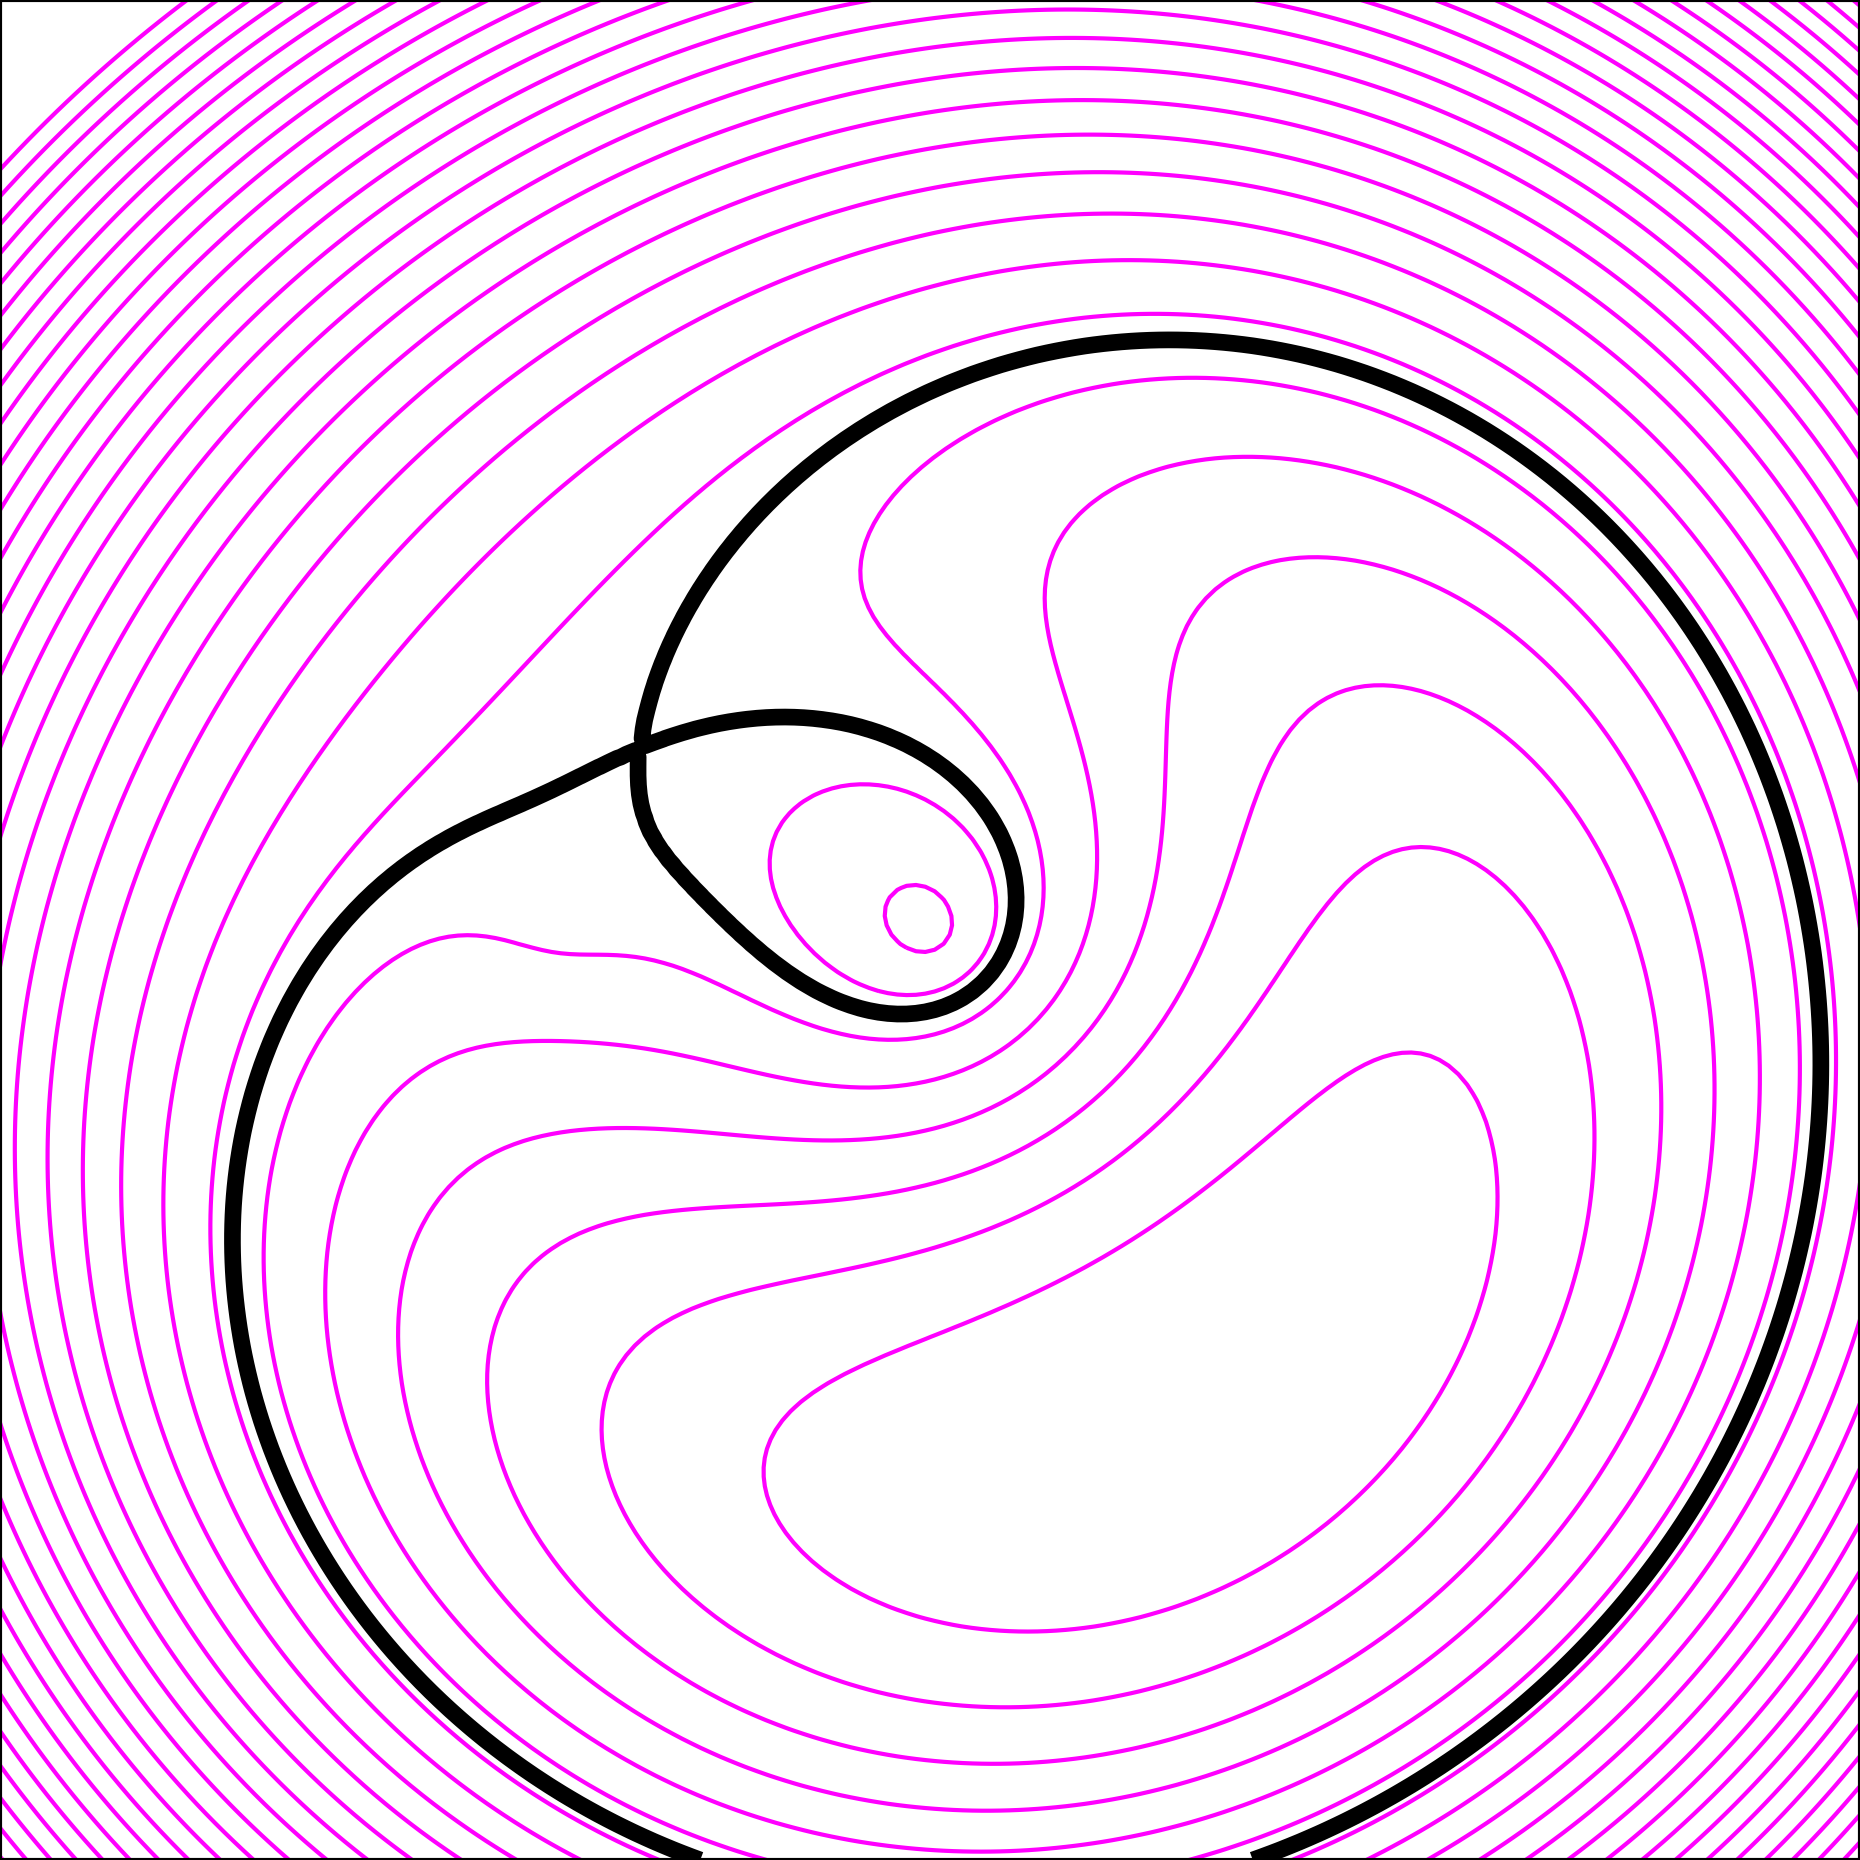
\includegraphics[width=\myplotswidth]{fig/ASW000195x_006975_arriv.png}
  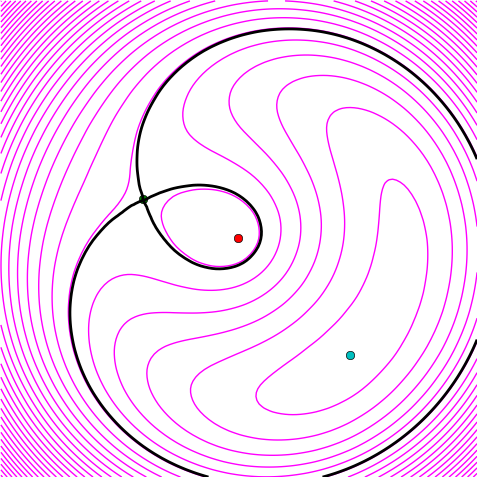
\includegraphics[width=\myplotswidth]{fig/006975_spaghetti} \\
  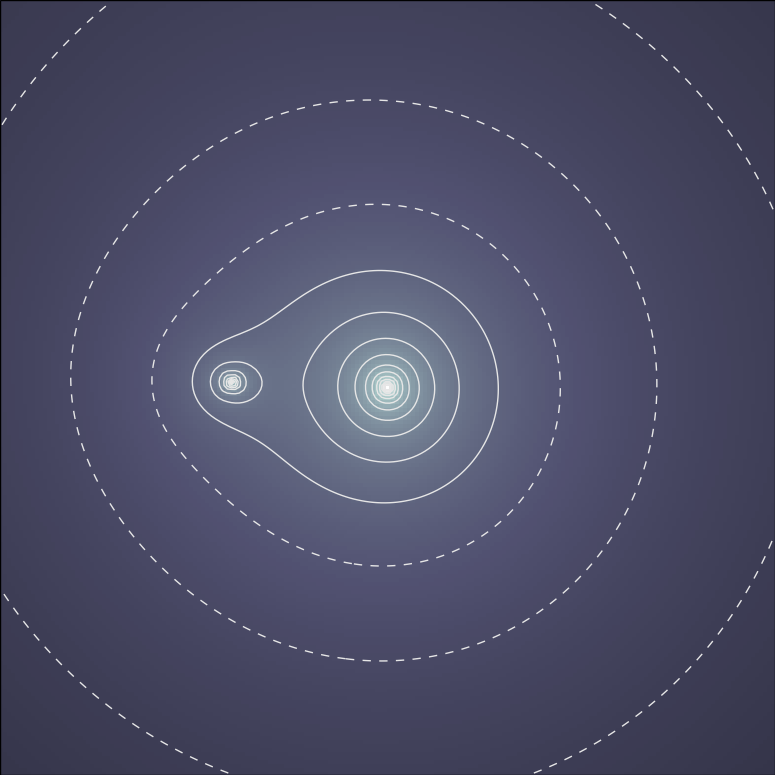
\includegraphics[width=\myplotswidth]{fig/ASW000195x_006975_kappa.png}
  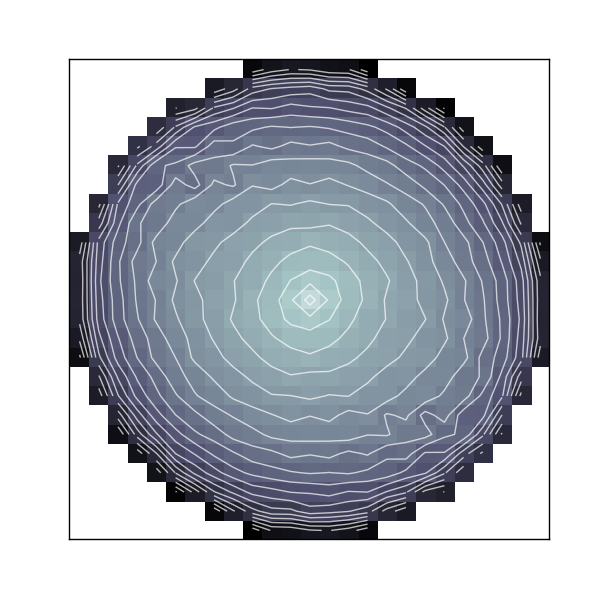
\includegraphics[width=\myplotswidth]{fig/006975_mass}
  \caption[result 6975 (ASW000195x)]{A lens with unrecovered mass
    substructure. (See Section \ref{sec:example_models} for details.)}
  \label{fig:6975}
\end{figure}
  
\begin{figure}
  \centering

  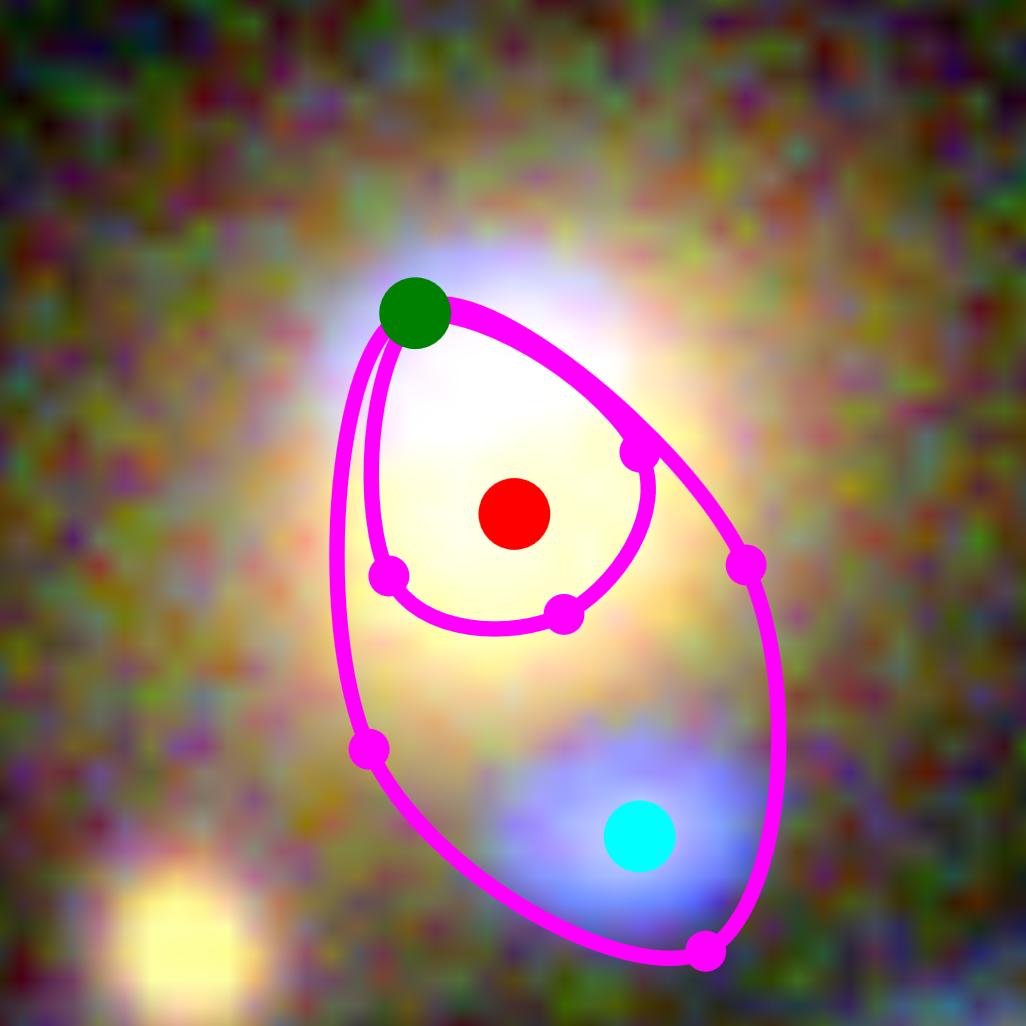
\includegraphics[width=\myplotswidth]{fig/006937_input}
  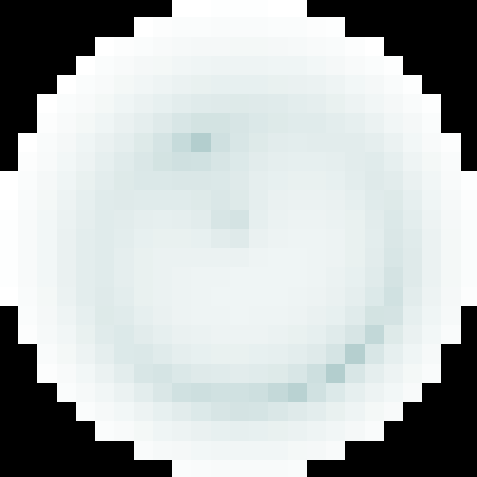
\includegraphics[width=\myplotswidth]{fig/006937_arr_time} \\
  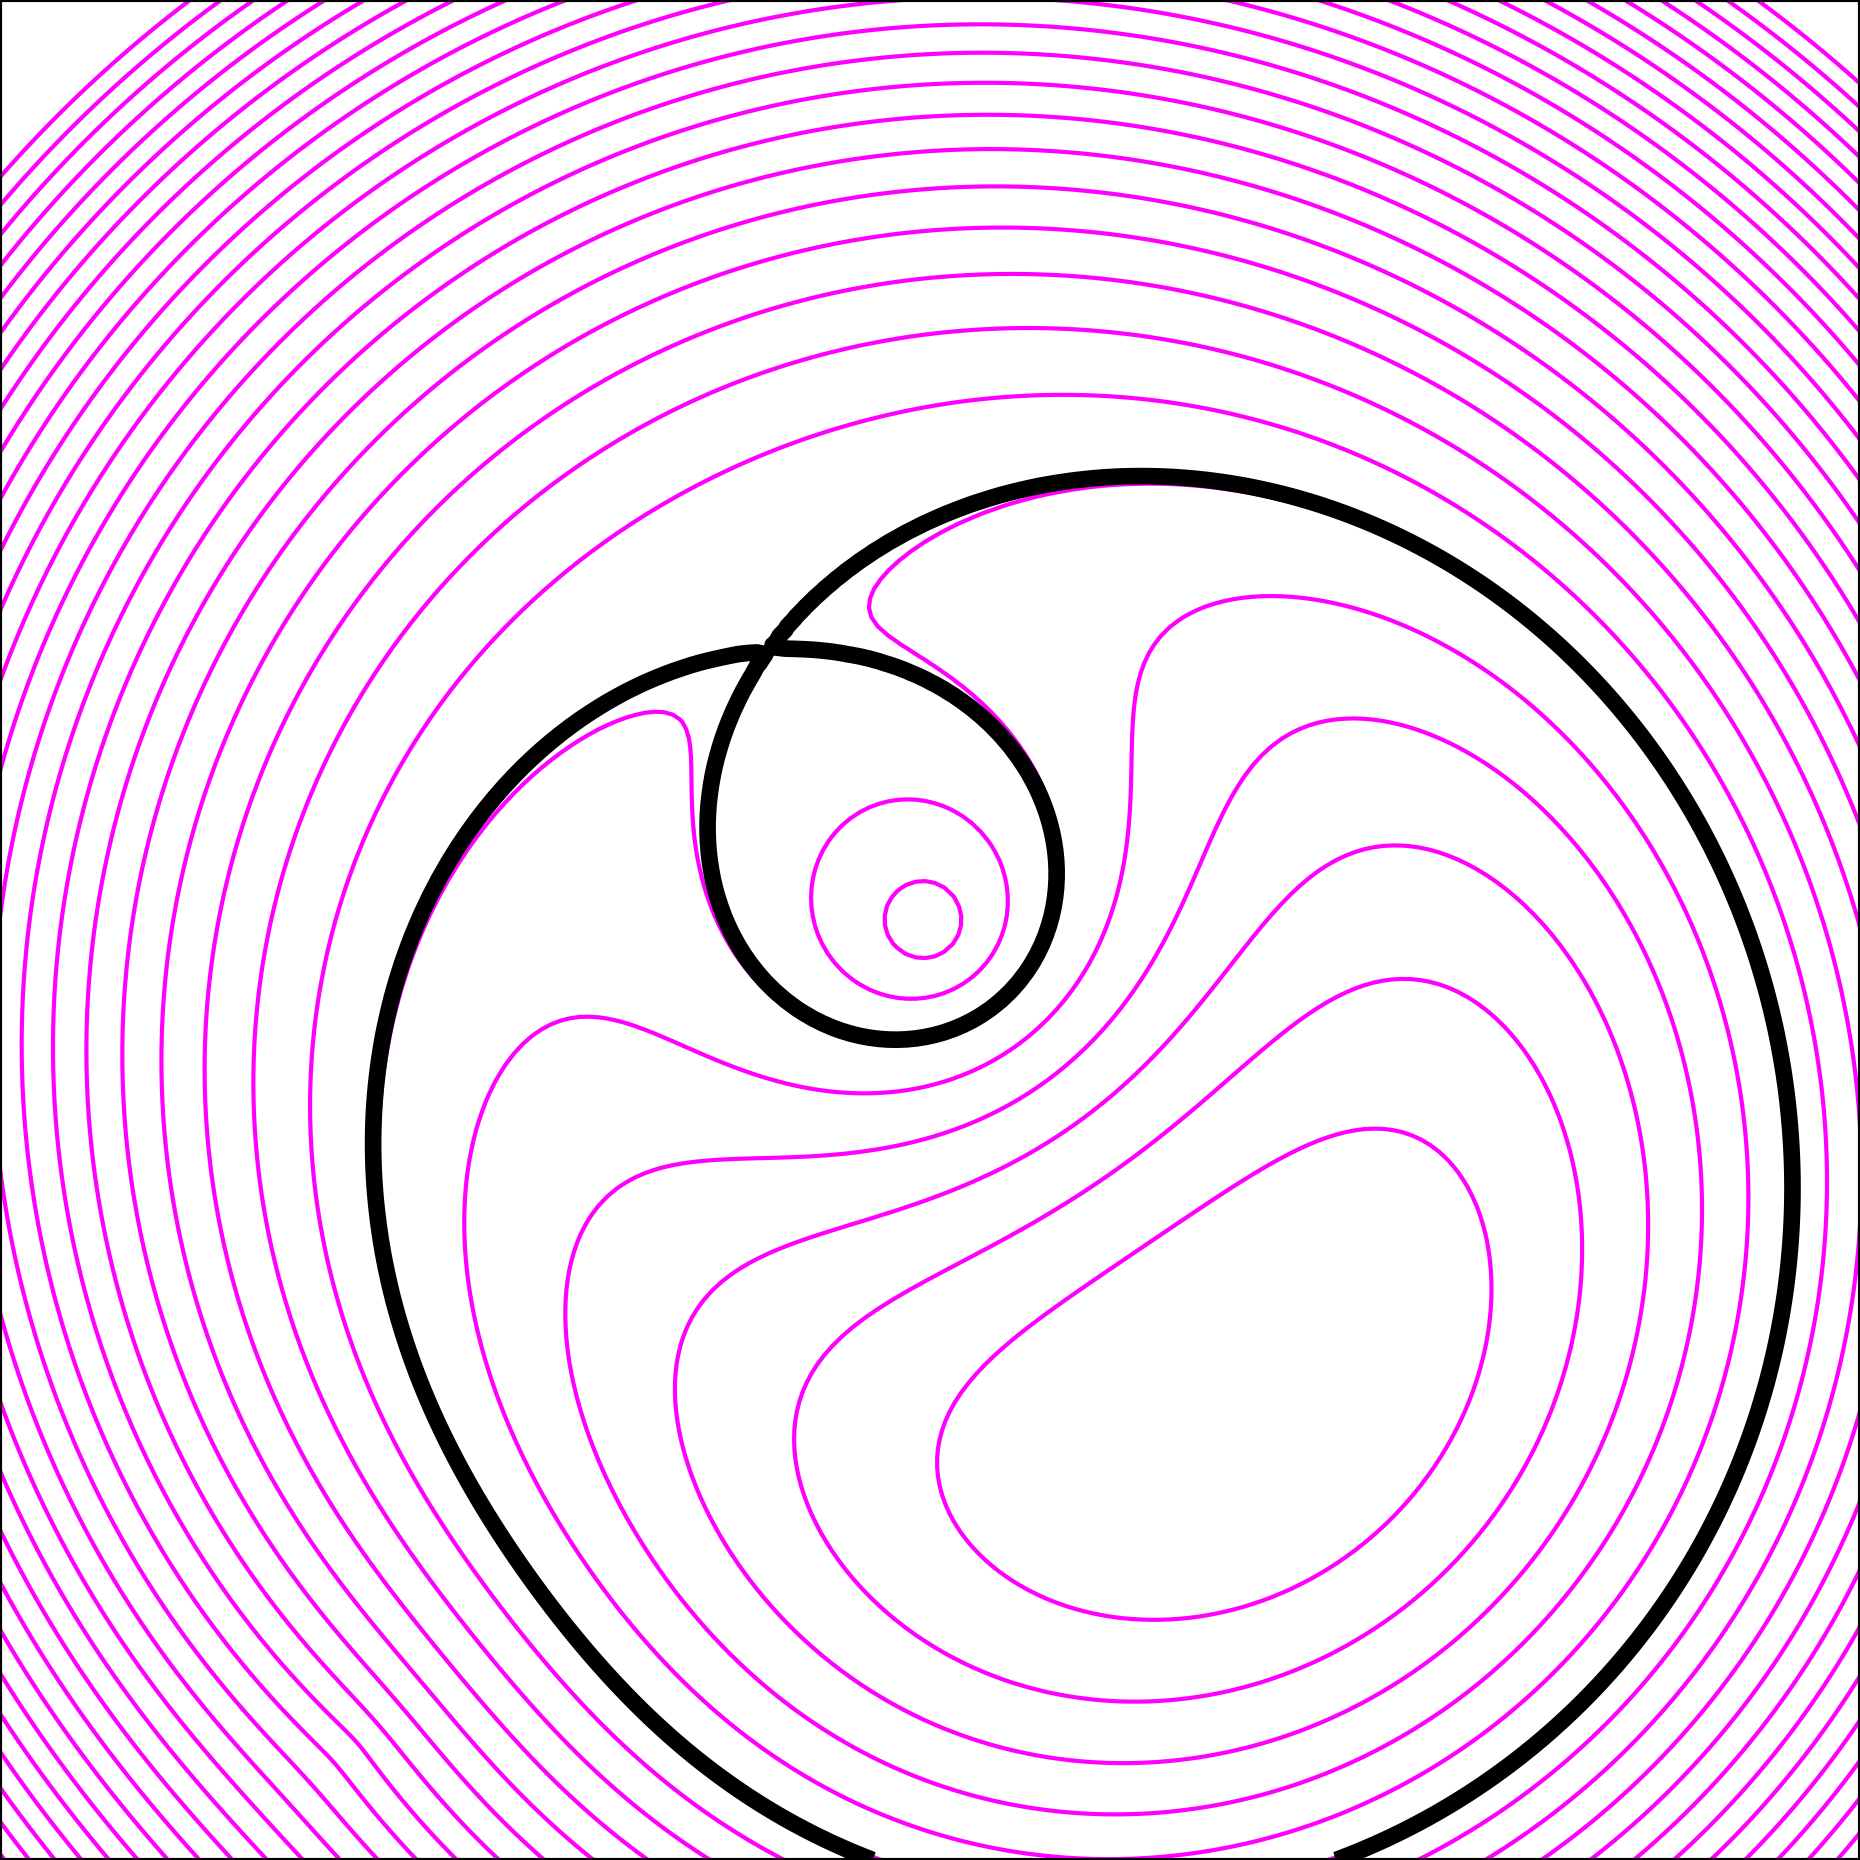
\includegraphics[width=\myplotswidth]{fig/ASW0000vqg_006937_arriv}
  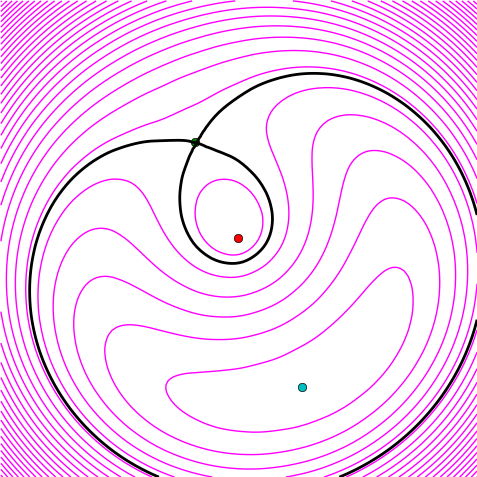
\includegraphics[width=\myplotswidth]{fig/006937_spaghetti} \\
  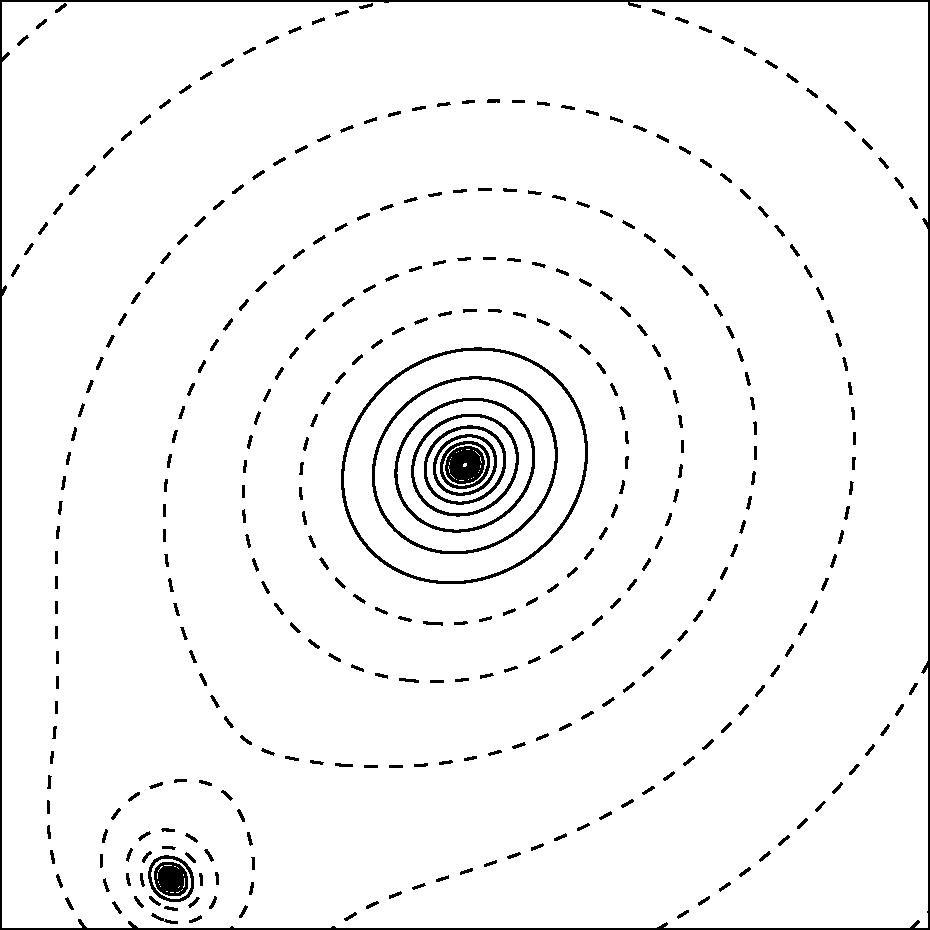
\includegraphics[width=\myplotswidth]{fig/ASW0000vqg_006937_kappa}
  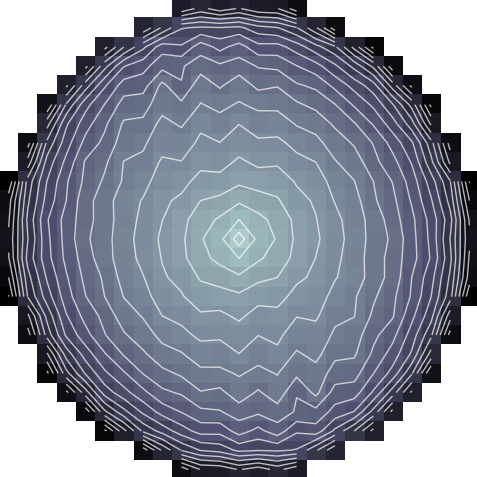
\includegraphics[width=\myplotswidth]{fig/006937_mass}

  \caption[result 6937 (ASW0000vqg)]{A sim with unrecovered
    substructure, resulting in a poor mass model. (See Section
    \ref{sec:example_models} for details.)}
  \label{fig:6937}
\end{figure}

\begin{figure}
  \centering

  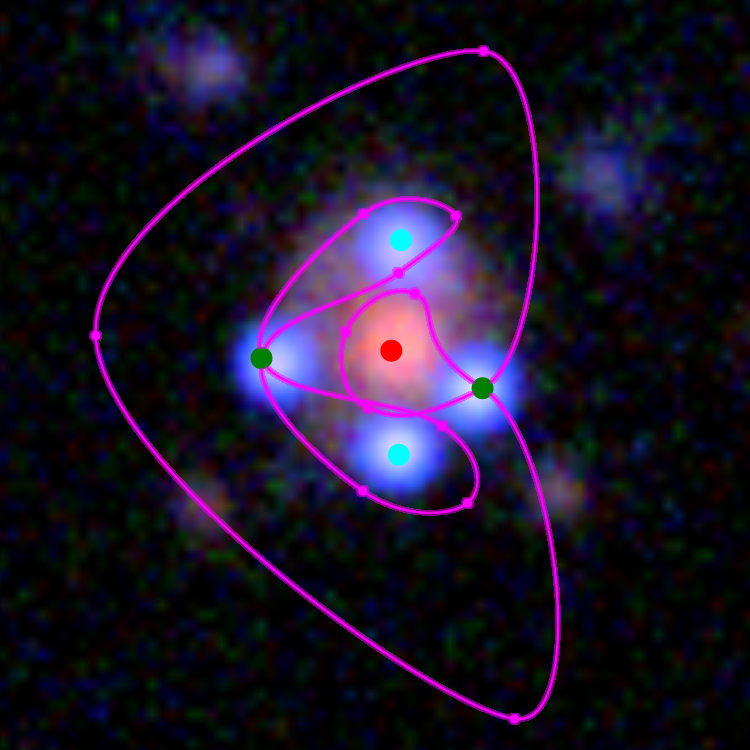
\includegraphics[width=\myplotswidth]{fig/007025_input}
  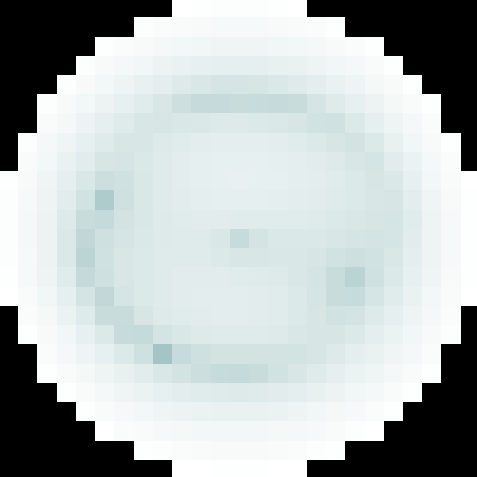
\includegraphics[width=\myplotswidth]{fig/007025_arr_time} \\
  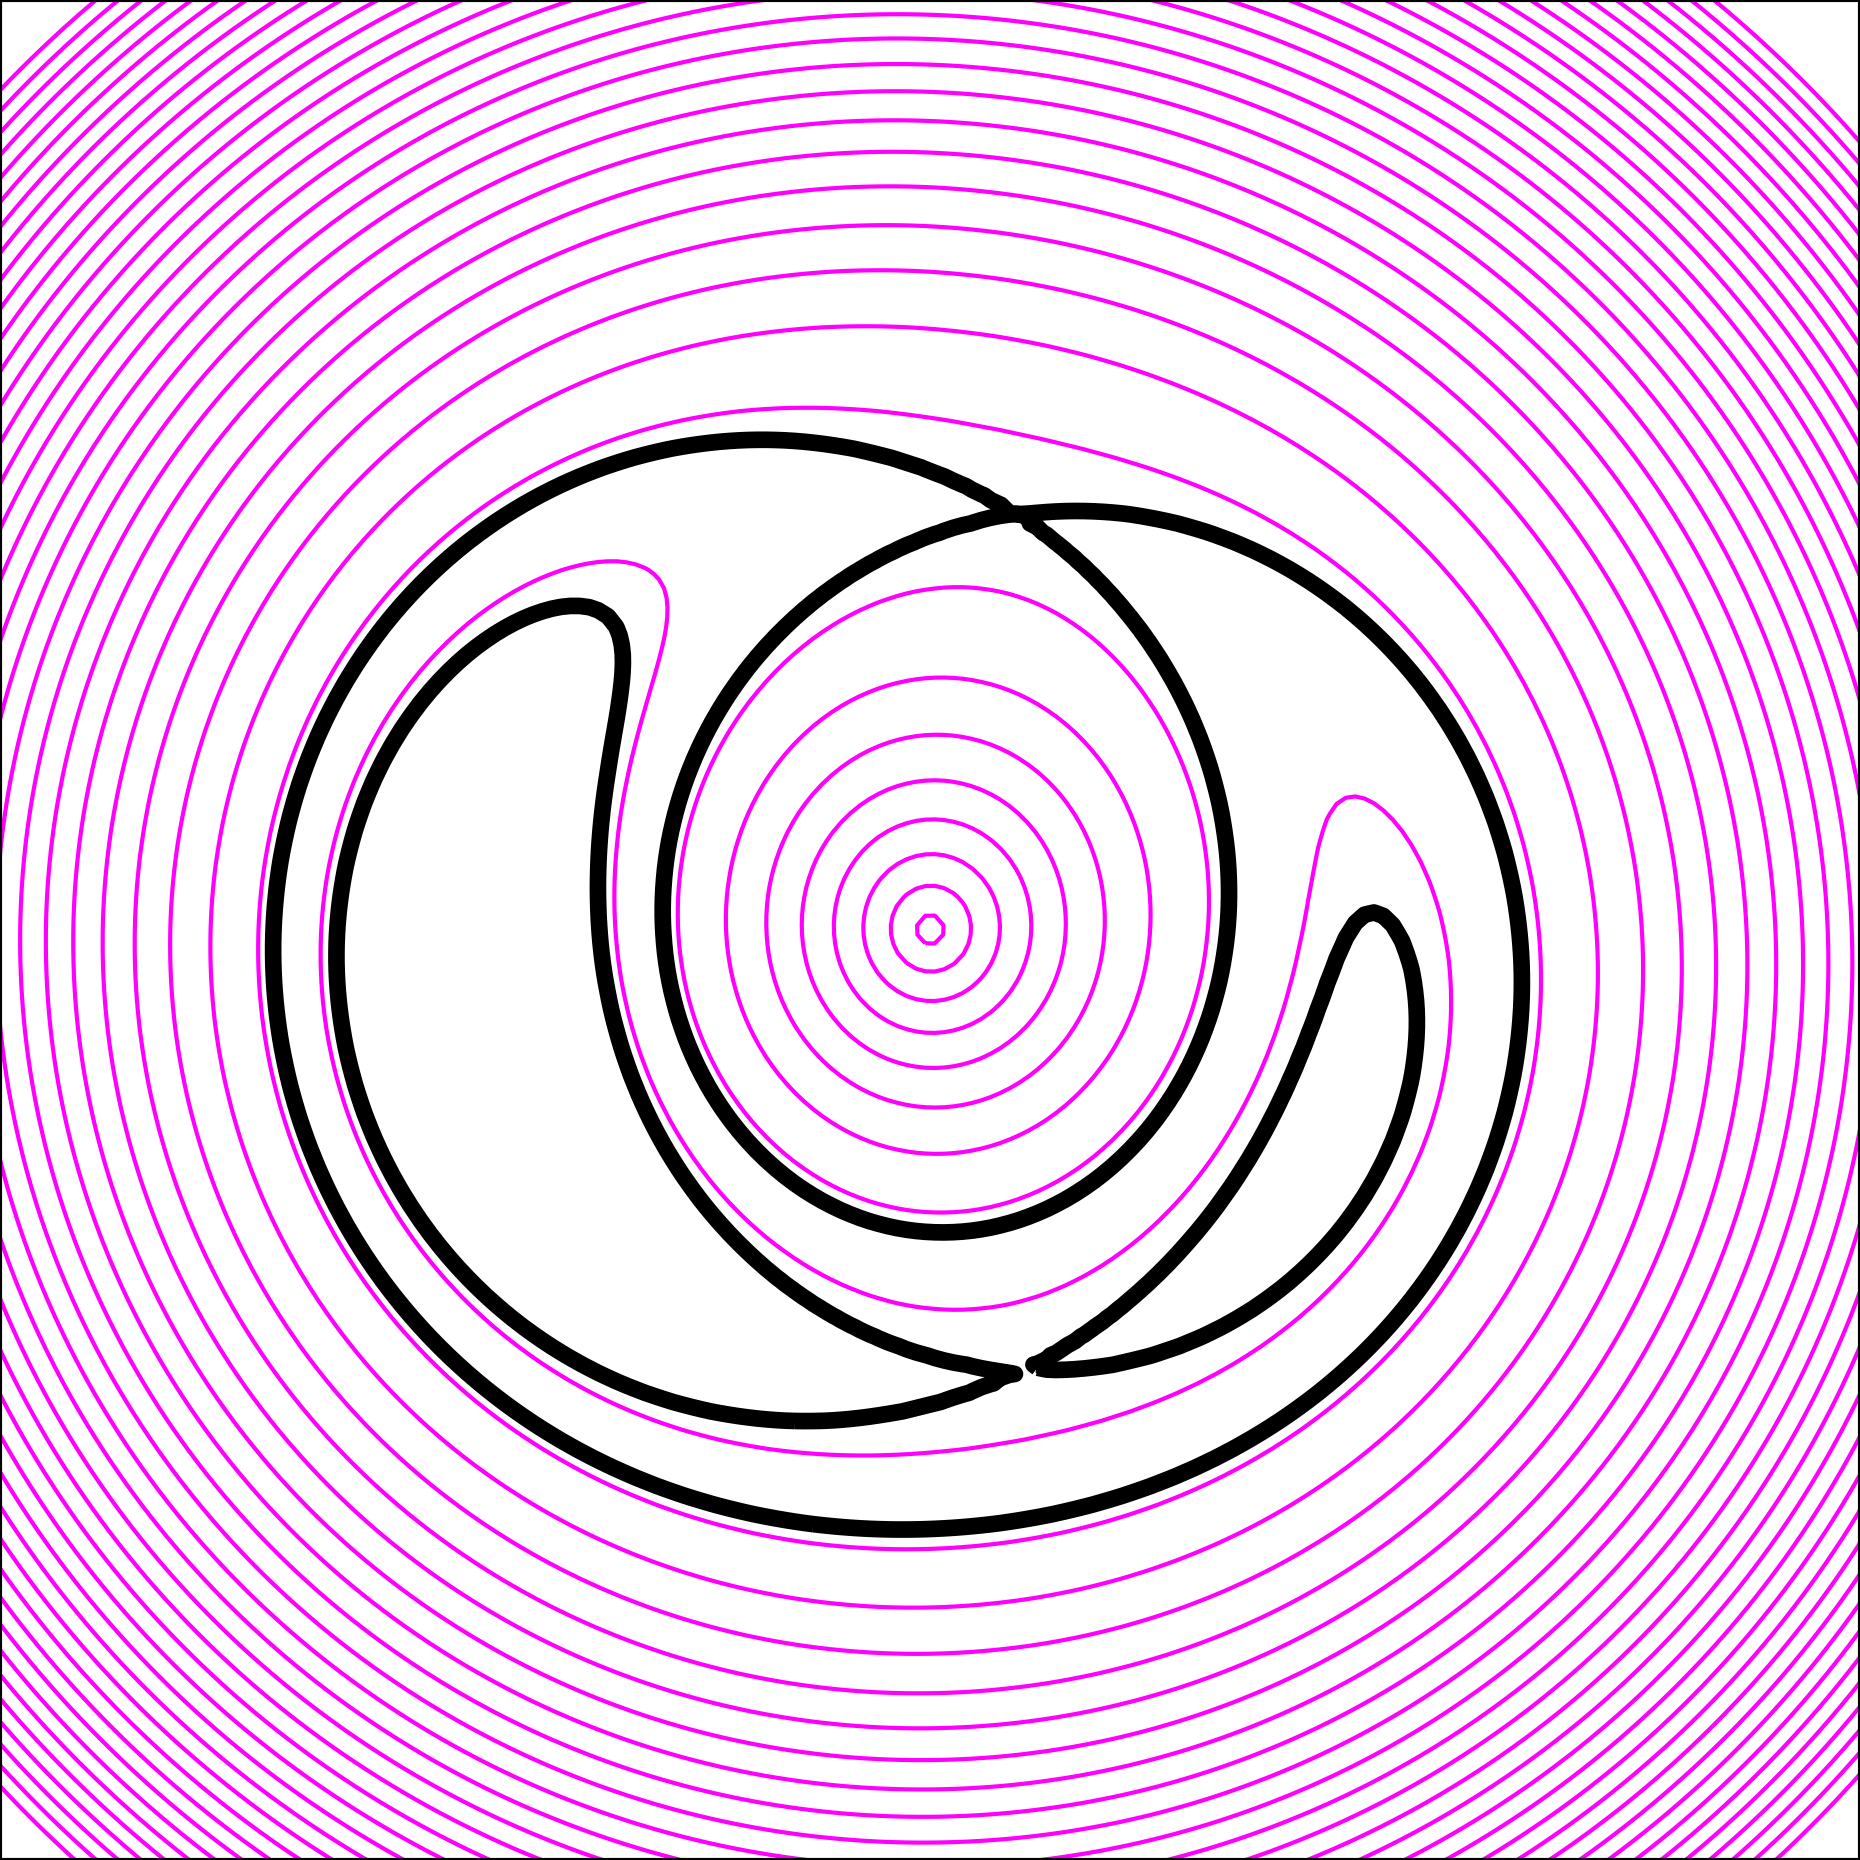
\includegraphics[width=\myplotswidth]{fig/ASW0000h2m_007025_arriv}
  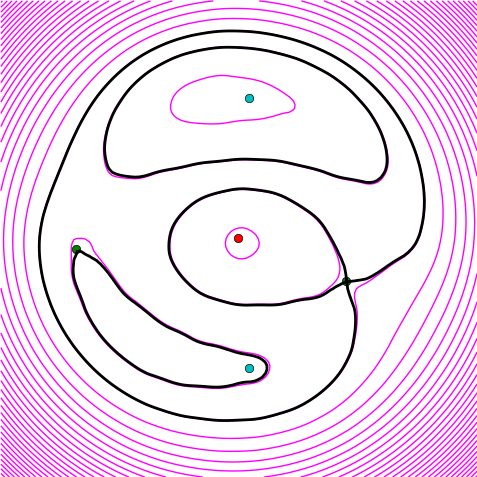
\includegraphics[width=\myplotswidth]{fig/007025_spaghetti} \\
  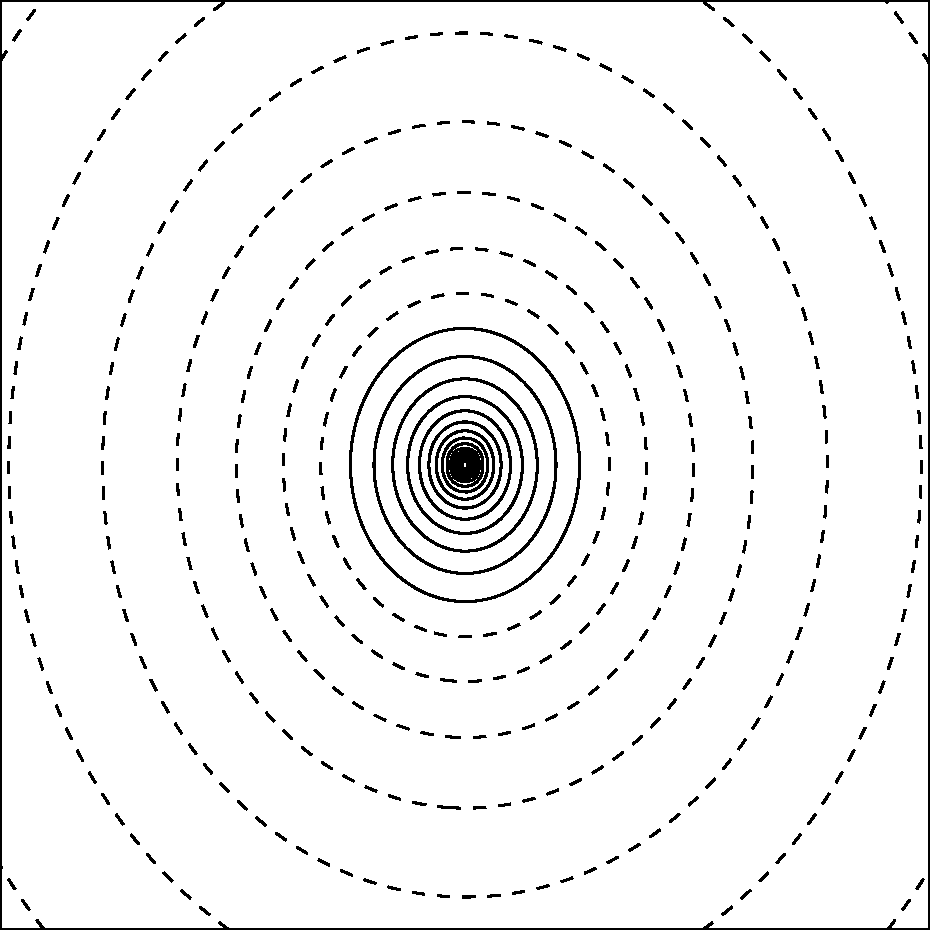
\includegraphics[width=\myplotswidth]{fig/ASW0000h2m_007025_kappa}
  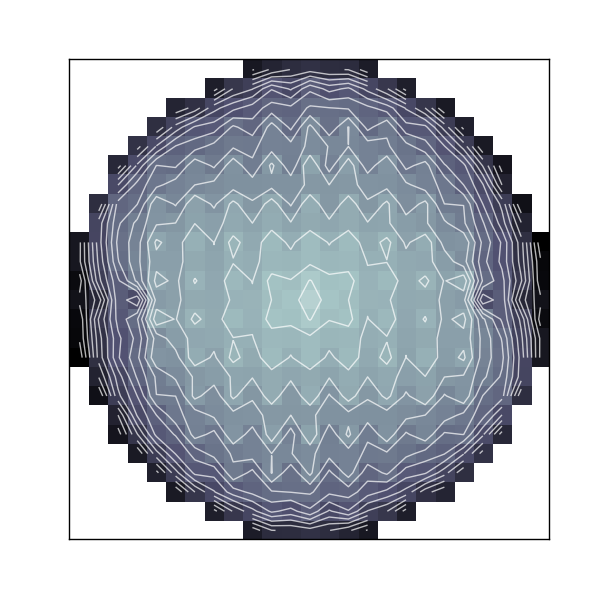
\includegraphics[width=\myplotswidth]{fig/007025_mass}
  \caption[result 7025 (ASW0000h2m)]{A four-image system with image
    parities incorrectly identified.  The model is poor, but the
    estimated Einstein radius is not bad. (See Section
    \ref{sec:example_models} for details.)}
  \label{fig:7025}
\end{figure}

\begin{figure}
  \centering


  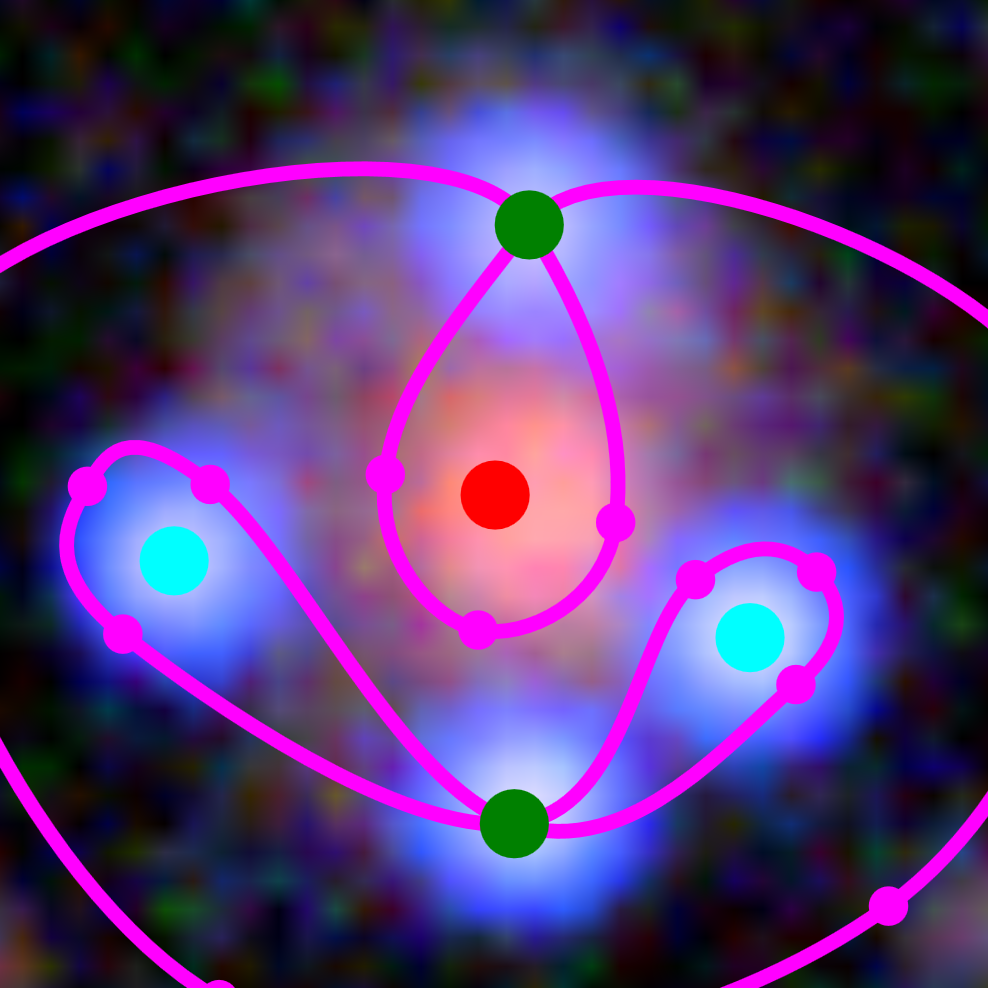
\includegraphics[width=\myplotswidth]{fig/007022_input}
  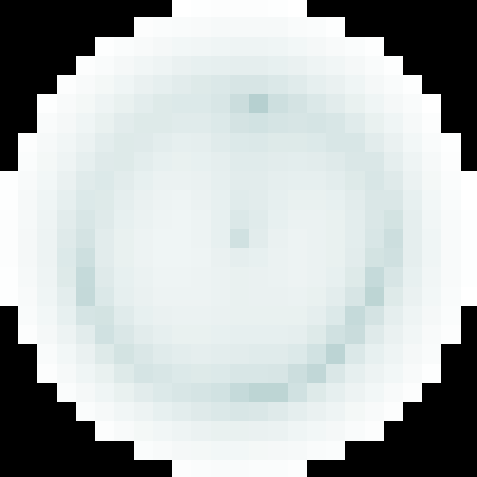
\includegraphics[width=\myplotswidth]{fig/007022_arr_time} \\
  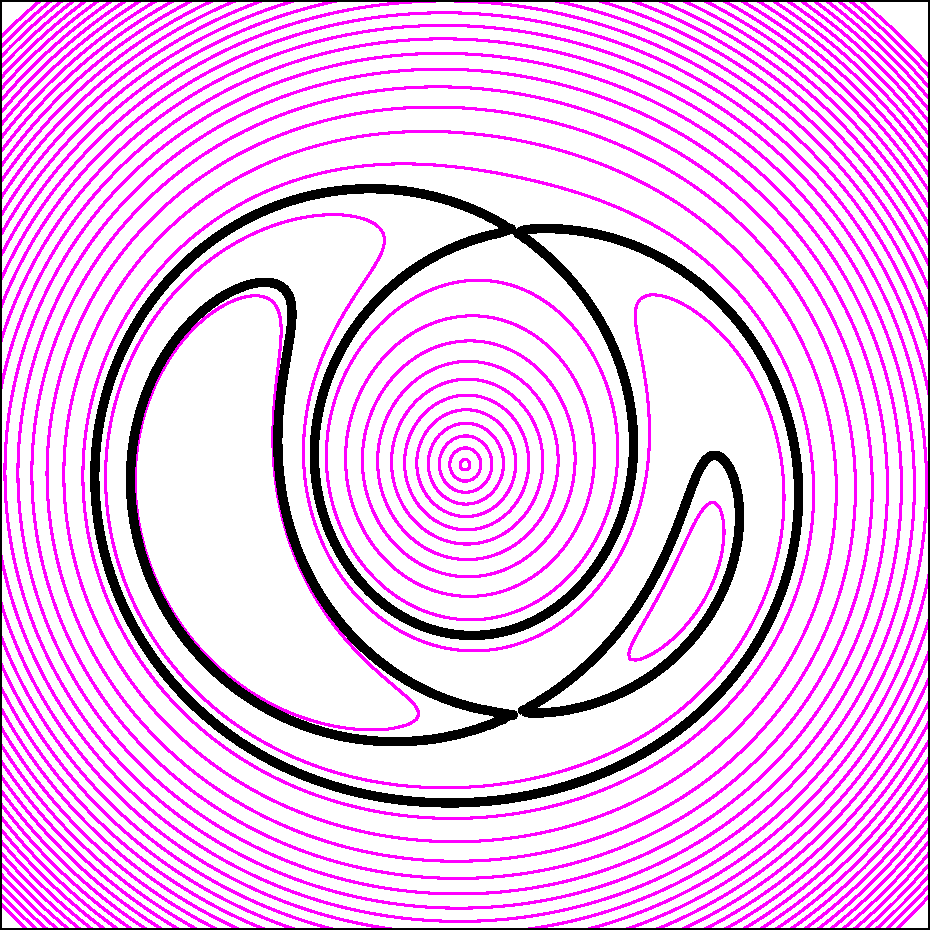
\includegraphics[width=\myplotswidth]{fig/ASW0000h2m_007022_arriv}
  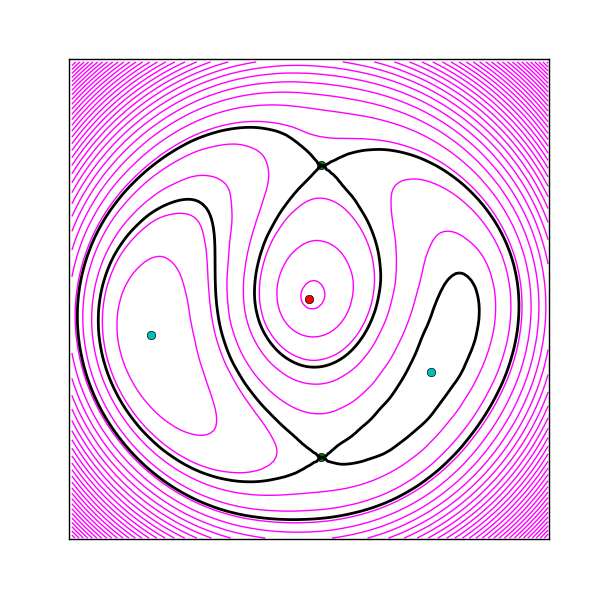
\includegraphics[width=\myplotswidth]{fig/007022_spaghetti} \\
  \includegraphics[width=\myplotswidth]{fig/ASW0000h2m_007022_kappa}
  \includegraphics[width=\myplotswidth]{fig/007022_mass}

  \caption[result 7022 (ASW0000h2m)]{The same system as in Figure
    \ref{fig:7025}, this time with image parities correctly
    identified. (See Section \ref{sec:example_models} for details.)}
  \label{fig:7022}
\end{figure}

\FloatBarrier

Figures \ref{fig:6941}--\ref{fig:7022} show details of eight models.
The first four of these show the most common image morphologies, the
other four explain some problem cases.  Each of the figures has the
following layout.
$$ \begin{matrix}
\hbox{marked-up image} \qquad &\hbox{model synthetic image} \\
t(x,y)                        &\hbox{model } t(x,y) \\
\kappa(x,y)                   &\hbox{model } \kappa(x,y)
\end{matrix} $$
The marked-up image is a zoom of the lensed image on Spacewarps,
marked up with one or more spaghetti contours; this is the modeller's
input to \spl.  The three panels on the right show the graphical
output returned to the modeller by \spl, listed as (i), (ii), (iii) in
\S\ref{sec:SpaghettiLens}).  These derive from the mean of an ensemble
of 200 models generated by \spl.

Figure \ref{fig:6941} shows a simple example.  In summary: the
identification of minimum and saddle point is correct, but the
estimated Einstein radius is a little too high.

Figure \ref{fig:6915} shows another quad.  This kind of configuration
arises when the mass is elongated and the source is displaced at an
angle to the elongation.

Figure \ref{fig:6990} shows an example of an arc that has split into
three images.  This kind of configuration, with a counter-image close
to the lensing galaxy and a more distant arc/triplet on the other
side, generically arises from an elongated mass distribution when the
source is displaced along the elongated direction.

To conclude this set of examples, Figure \ref{fig:6919} shows another
type of quad.  Actually, in this case the brightest part of the source
is only doubly imaged, but the source extends into a region that
produces four images.  We can also see from the real arrival-time
surface that a point source is a double on the verge of splitting into
a quad.  The modeler interpreted the system as a quad.  The
appearance of the arcs, shown in the bottom panel of Figure
\ref{fig:input-spag}, looks like an arc and counter-image such as
discussed with Figure \ref{fig:6990} above.  But there is an important
difference: the long arc is closer to the galaxy, as if the arc and
counter-image have swapped roles.  This configuration arises if the
source displacement is perpendicular to the long axis of the lensing
mass.


Figure \ref{fig:6975} shows a lens with substructure in the form of a
smaller secondary galaxy.  The galaxies in such group or cluster sims
were, in fact, based on galaxies visible in the images --- but the
modelers were not told in advance whether this was the case.  The
model does not include any substructure, but otherwise is not bad.
The minimum and saddle point are correct, and the Einstein radius is
only a little underestimated.

Figure \ref{fig:6937} shows a case where substructure leads to a
poor model.


Figure \ref{fig:7022} shows another model of the same system.  In this
one, the identification of the minima and saddle points was incorrect,
and mass distribution comes out elongated East-West instead of
North-South.  The mass distribution also appears somewhat jagged and
the saddle-point contours are not as clean as in the previous
examples; these are often indicators of a problem with the model.  The
enclosed mass is, however, none the worse --- the reason is probably
that in a relatively symmetrical image configuration, the Einstein
radius is quite well constrained by the images in a fairly
model-independent way.


Figure \ref{fig:6975} shows a fairly symmetric quad.  The minima and
saddle points are correctly identified, and the orientation of the
ellipticity of the mass distribution is correctly reproduced.  The
Einstein radius is somewhat overestimated.  

Figure \ref{fig:kapenc_compare_faulty} shows a comparison of input and
recovered mass profiles.  The panel shows a average $\kappa$ within a
given radius, as a function of radius.  The red curve is the true
value, and where it crosses unity (dotted horizontal line) is the
notional Einstein radius $\Theta_{\text{E, sim}}$.  The two blue
curves are the minimal and maximal mean enclosed $\kappa$ from the
internal ensemble in \spl.  The region between the blue curves is
shaded between the radii of the innermost and the outermost images ---
this is the confidence region from the modeling.  As we see, the
shaded blue is slightly above the red curve.  The Einstein Radius
$\Theta_\text{E}$ of the model is estimated crossing the mean enclosed
$\kappa$ (not plotted) with unity.


The panel shows
a average $\kappa$ within a given radius, as a function of radius.
The red curve is the true value, and where it crosses unity (dotted
horizontal line) is the notional Einstein radius $\Theta_{\text{E, sim}}$.
  The two blue curves
are the minimal and maximal mean enclosed $\kappa$ from the internal
ensemble in \spl.  The region between the blue curves is shaded
between the radii of the innermost and the outermost images --- this
is the confidence region from the modeling.  As we see, the shaded
blue is slightly above the red curve. 
The Einstein Radius $\Theta_\text{E}$ of the model is estimated crossing the
mean enclosed $\kappa$ (not plotted) with unity.
